\chapter{Progettazione}

\label{cap:progettazione}

\intro{Durante la fase di progettazione viene definita l'architettura del software, questa operazione consiste nella suddivisione del sistema in componenti distinti, ognuno con compiti differenti.
L'obiettivo è pianificare in maniera chiara tutte le azioni che l'applicativo dovrà svolgere prima di passare effettivamente alla codifica.}

\section{Architettura}
L'architettura (Fig.~\ref{fig:schema-architettura}) pensata prevede l'utilizzo di 4 componenti principali che si occupano di:
\begin{enumerate}
    \item Acquisire gli screenshot.
    \item Effettuare il \emph{clustering} degli screenshot acquisiti.
    \item Valutare i siti web.
    \item Inviare e-mail promozionali.
\end{enumerate}
La suddivisione in componenti consente di avere un codice più strutturato e specializzato nell'assolvimento di determinati compiti; rende anche la comprensione da parte di altri programmatori più rapida e chiara.
I vari moduli comunicano con il database di SalesCRM attraverso l'utilizzo di \gls{API} che eseguono interrogazioni e inserimenti.
Nel caso della comunicazione tra il modulo di \emph{clustering} e quello di valutazione la condivisione di dati avviene in maniera diretta utilizzando la memoria dello stesso PC; questa modalità non si rivela problematica poiché garantisce uno scambio rapido di informazioni che deve essere svolto solo ed esclusivamente in fase di addestramento.

\begin{figure}[!h] 
    \centering 
    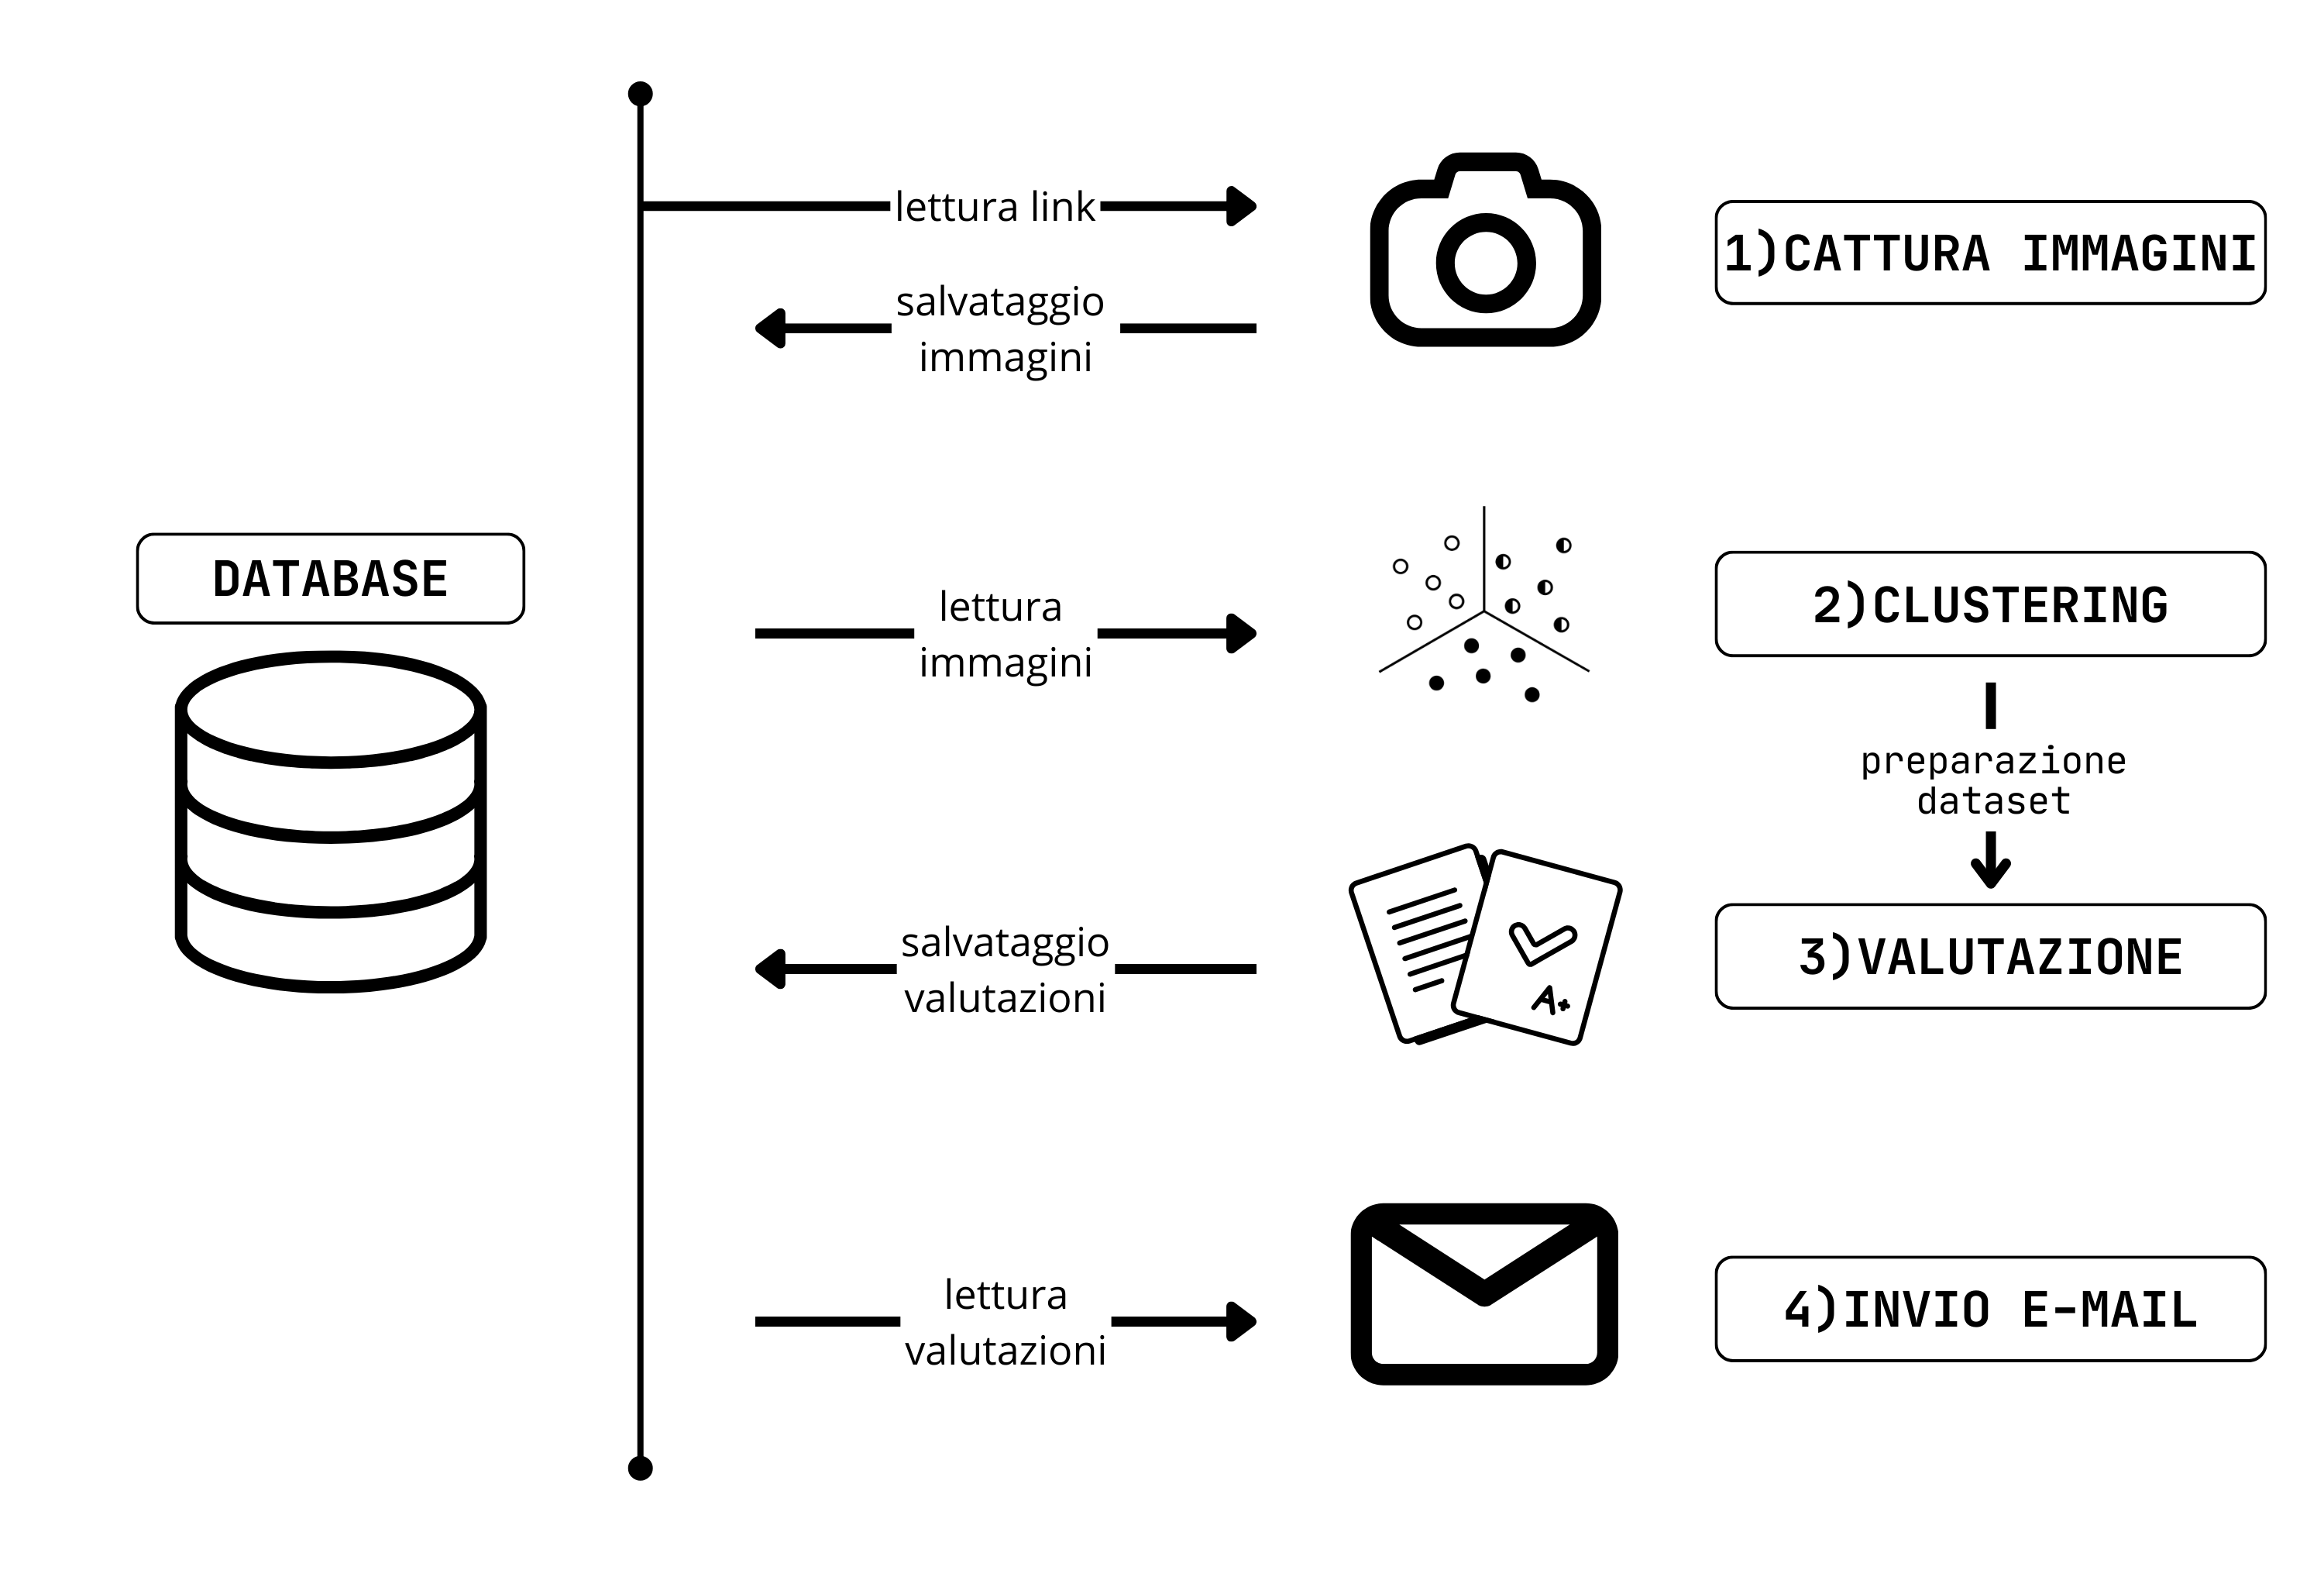
\includegraphics[width=0.9\columnwidth]{progettazione/schema-architettura.png} 
    \caption{Schema architetturale del progetto}
    \label{fig:schema-architettura}
  \end{figure}


\newpage

\section{Cattura immagini}
La prima fase del \emph{\gls{workflow}} (Fig.~\ref{fig:schema-cattura}) è composta da uno script Python che usufruisce della libreria Pyppeteer per acquisire gli screenshot dei siti contenuti nel database.
Più precisamente un \emph{web scraper} già implementato raccoglie i link delle pagine web dei clienti potenziali, successivamente li carica nel database di SalesCRM, dove verranno infine letti dallo script.
Per funzionare Pyppeteer necessita di chromium, dopo aver effettuato il controllo per verificare se esso sia presente o meno procede con la lettura dei link. 
L'automazione apre ogni indirizzo, aspetta qualche secondo e scatta uno screenshot. 
Tutte le immagini vengono poi convertite in formato Base64 per adattarsi alle tabelle già esistenti e salvate nel database.

\begin{figure}[!h] 
  \centering 
  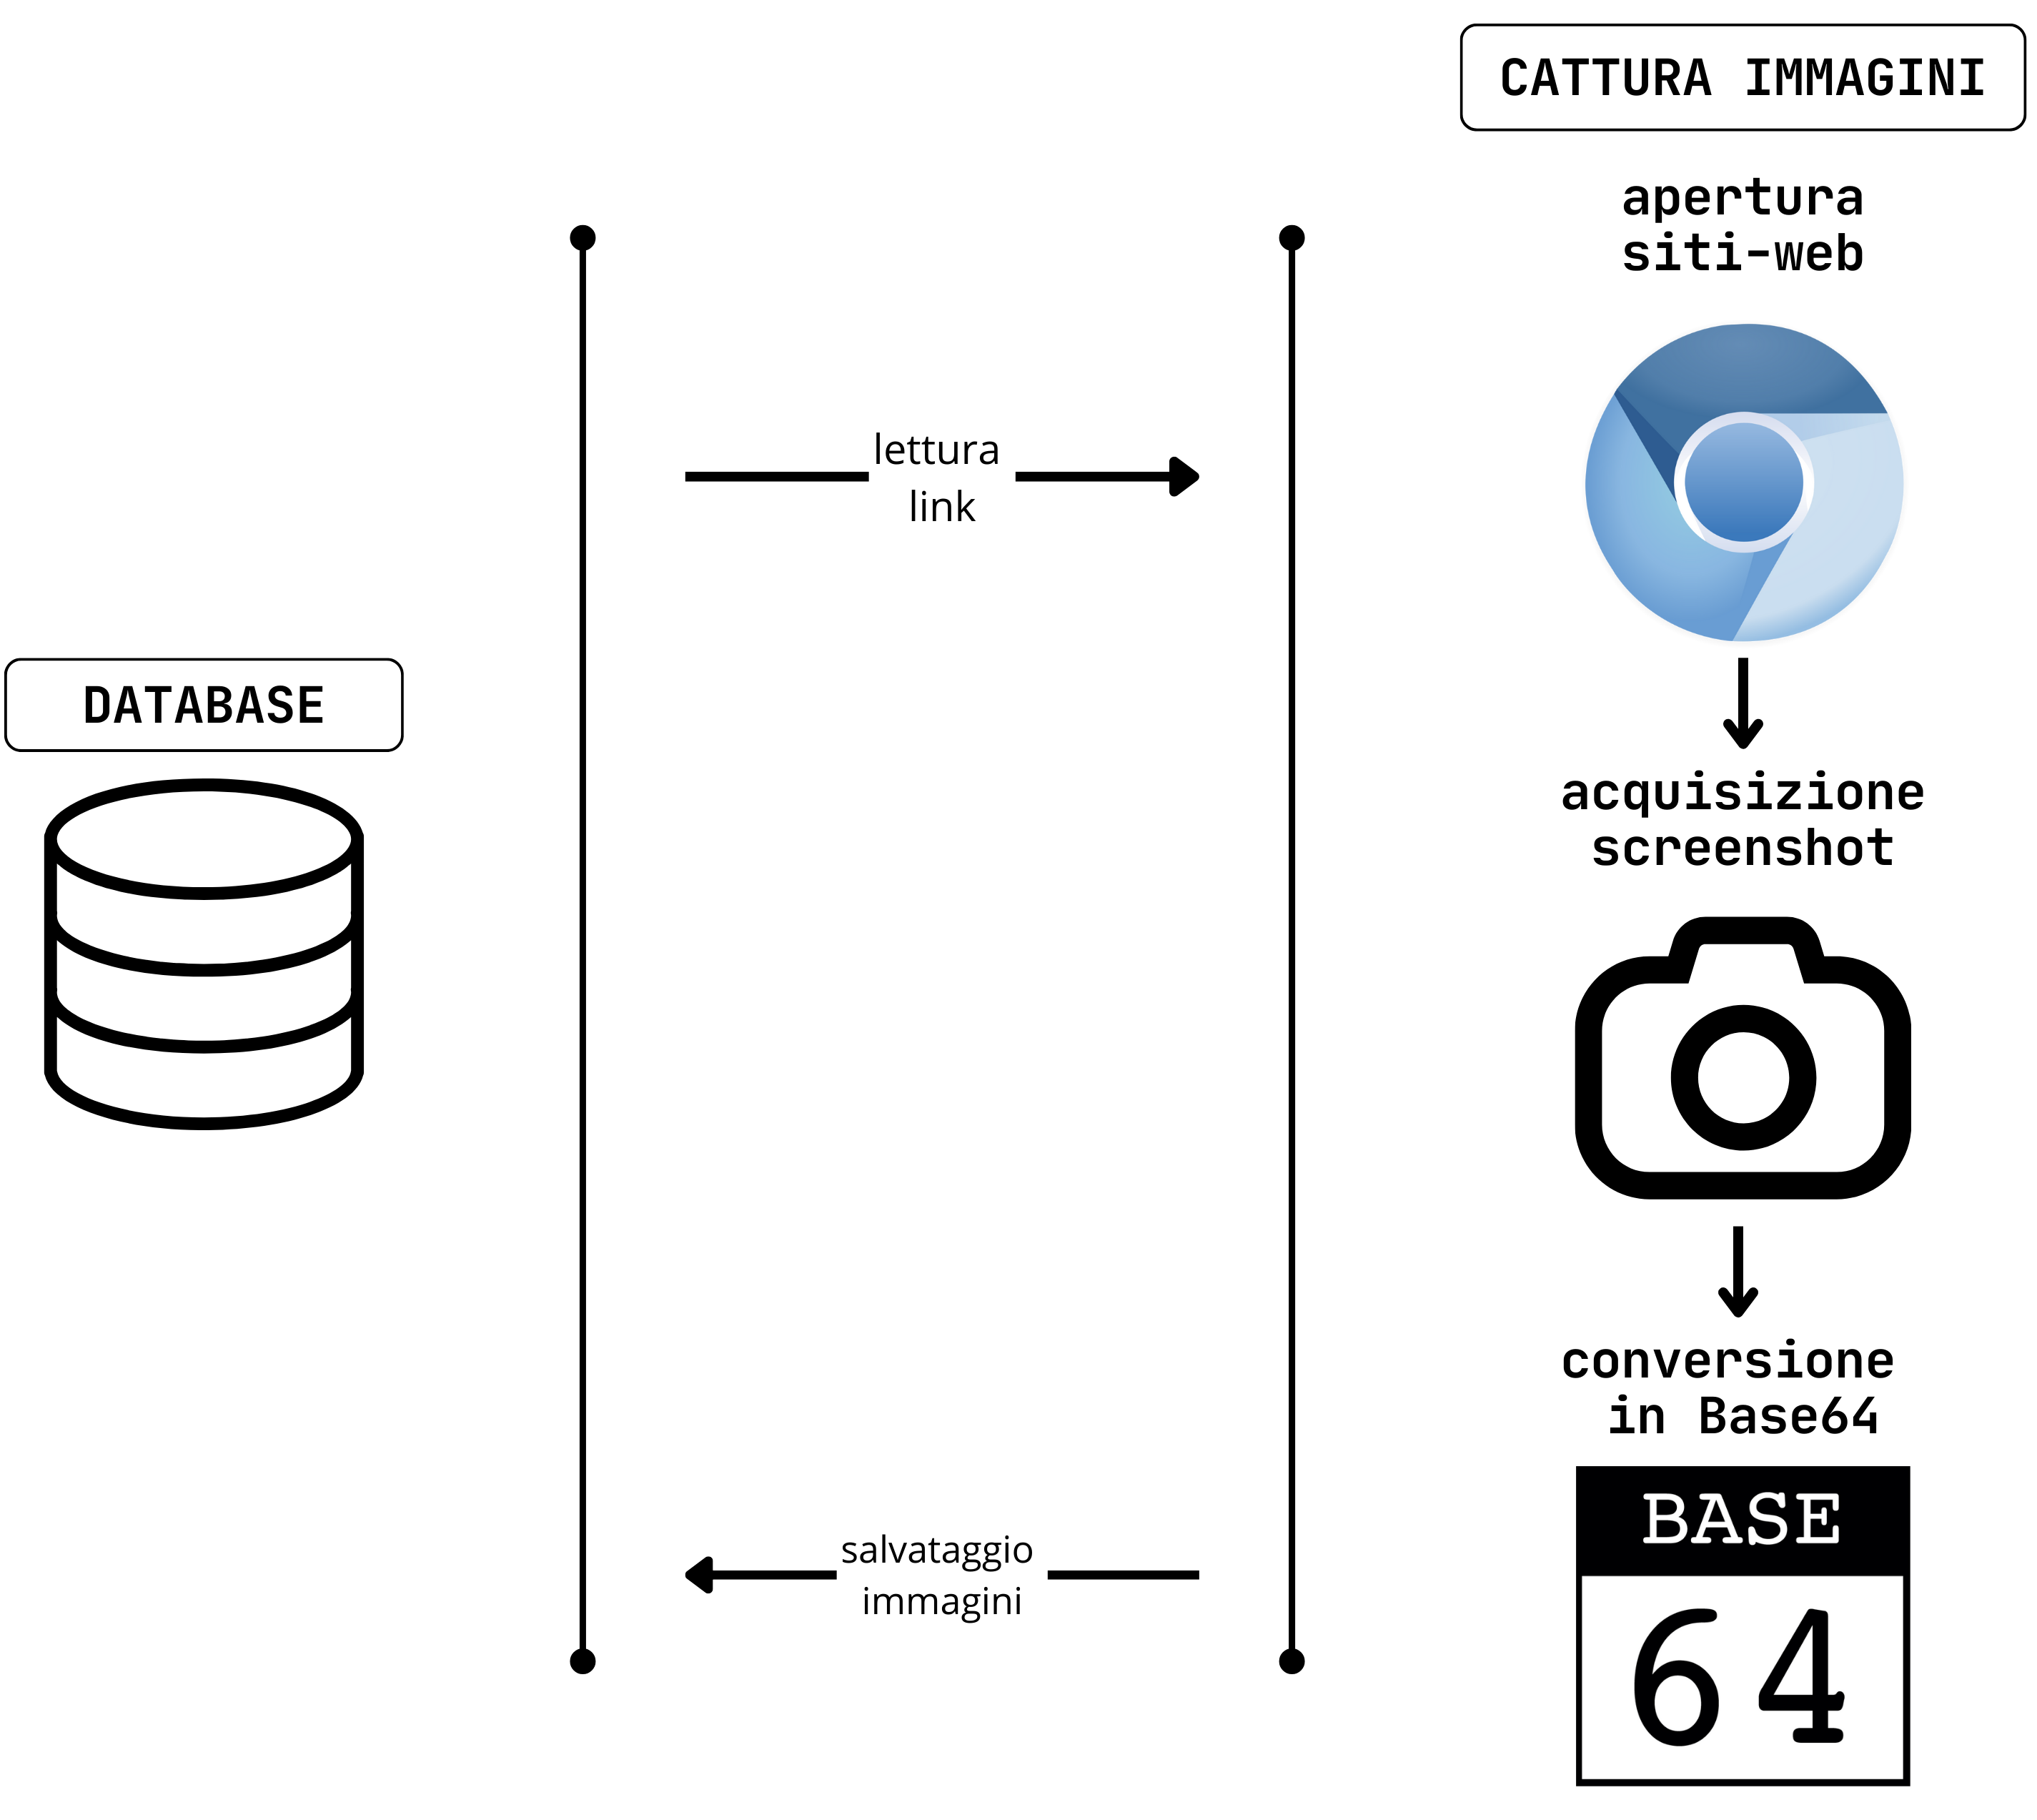
\includegraphics[width=0.5\columnwidth]{progettazione/schema-cattura.png} 
  \caption{Schema della fase di cattura}
  \label{fig:schema-cattura}
\end{figure}

\newpage

\section{Studio preliminare per l'estrazione delle feature}
L'estrazione delle \emph{\gls{feature}} è una fase fondamentale e necessita pertanto di uno studio più approfondito.

\subsection{Tentativi con autoencoder}
Gli \emph{autoencoder} sono stati utilizzati inizialmente poiché si pensava che la soluzione migliore fosse la creazione di un modello \emph{CNN} che si adattasse completamente alle \emph{\gls{feature}} presenti nei siti web, ma si è rivelato particolarmente difficile per i motivi seguenti:
\begin{itemize}
  \item Numero elevato di epoche di addestramento.
  \item Studio della quantità e tipologia degli strati.
  \item Bilanciamento arduo tra dimensioni accettabili e memoria a disposizione.
\end{itemize}

\subsubsection{Autoencoder con soli strati densi}
Il primo tentativo è stato effettuato utilizzando un \emph{autoencoder} che sfrutta esclusivamente \emph{layer} densi (Fig.~\ref{fig:schema-denso}), questo metodo nonostante abbia portato a dei risultati si è rivelato problematico visto che per funzionare in maniera efficiente, senza richiedere una GPU troppo prestante, necessita di immagini in bianco e nero di dimensioni ridotte a 128*128 (Fig.~\ref{fig:dense-ricostruita}).

\begin{figure}[!h] 
  \centering 
  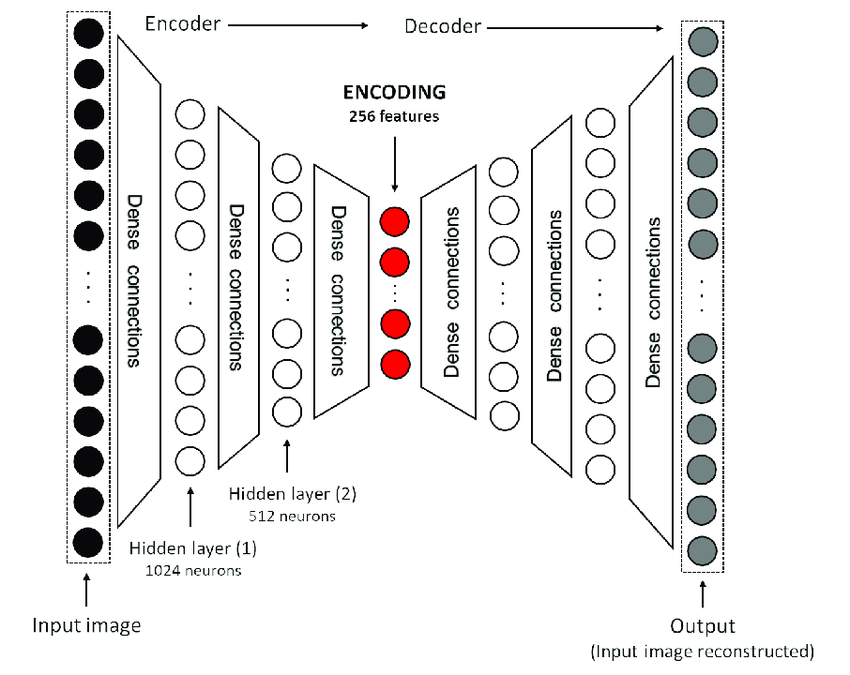
\includegraphics[width=0.6\columnwidth]{progettazione/autencoder_dense_layers.png} 
  \caption{Autoencoder con strati densi}
  \label{fig:schema-denso}
\end{figure}


\begin{figure}[!h] 
  \centering 
  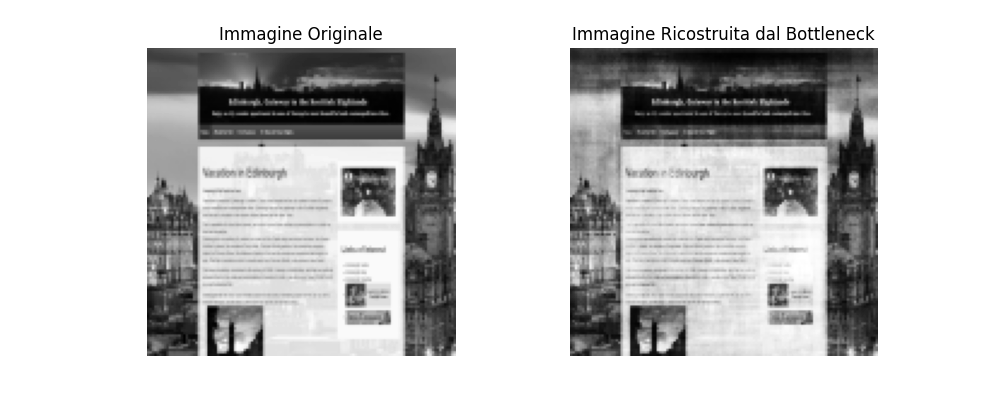
\includegraphics[width=1\columnwidth]{progettazione/dense_200Immagini_150Epoche_10BatchSize_BW.png} 
  \caption{Ricostruzione immagine ottenuta dal bottleneck dell'autoencoder a strati densi con 150 epoche di addestramento}
  \label{fig:dense-ricostruita}
\end{figure}

\newpage

\subsubsection{Autoencoder con strati convoluzionali}
L'\emph{autoencoder} con strati convoluzionali (Fig.~\ref{fig:schema-conv}) ha consentito un netto miglioramento delle prestazioni e un consumo inferiore della memoria tali da poter aumentare le dimensioni delle immagini e implementare nuovamente l'utilizzo del colore.
Le modifiche non sono state comunque sufficienti per avere un esperienza di utilizzo solida causando:
\begin{itemize}
  \item \emph{Overflow} della \emph{\gls{V-RAM}}\glsfirstoccur se non utilizzato sotto specifiche condizioni.
  \item Inconsistenza nei \emph{cluster}.
\end{itemize}
Viene sotto riportata un immagine in bianco e nero di dimensioni 256*256 ottenuta dal \emph{bottleneck} dell'\emph{autoencoder} per comparare con il modello precedente (Fig.~\ref{fig:conv-ricostruita}).

\begin{figure}[!h] 
  \centering 
  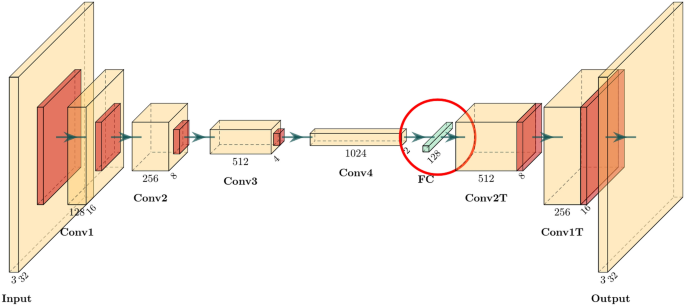
\includegraphics[width=0.7\columnwidth]{progettazione/Convolutional_autoencoder.png} 
  \caption{Autoencoder con strati convoluzionali}
  \label{fig:schema-conv}
\end{figure}


\begin{figure}[!h] 
  \centering 
  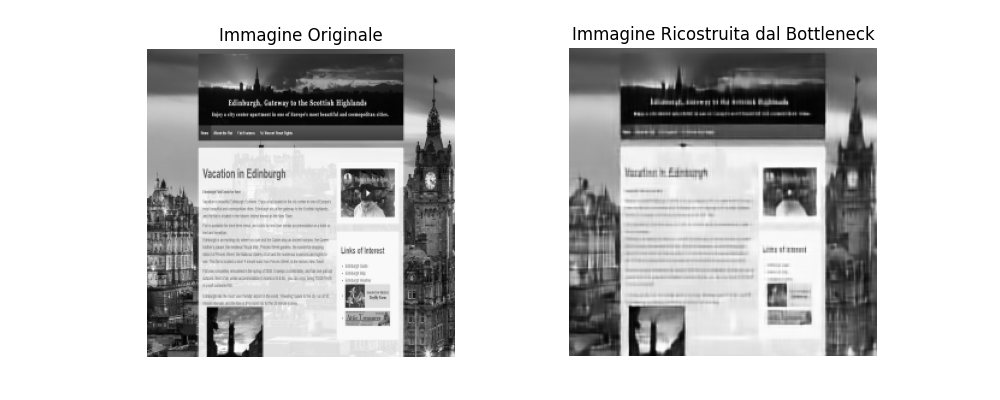
\includegraphics[width=1\columnwidth]{progettazione/Conv_BW_img_dim256Epochs500Batch32Images5000.png} 
  \caption{Ricostruzione immagine ottenuta dal bottleneck dell'autoencoder convoluzionale con 500 epoche di addestramento}
  \label{fig:conv-ricostruita}
\end{figure}

Un altro vantaggio dell'utilizzo di strati convoluzionali è la possibilità di visualizzare le \emph{feature map} estratte da ciascun \emph{layer} (Fig.~\ref{fig:conv-1}, Fig.~\ref{fig:conv-2}, Fig.~\ref{fig:conv-3}). Grazie a esse lo sperimentatore ha un'idea più chiara di quello che avviene all'interno dell'\emph{autoencoder}.


\begin{figure}[!htbp] 
  \centering 
  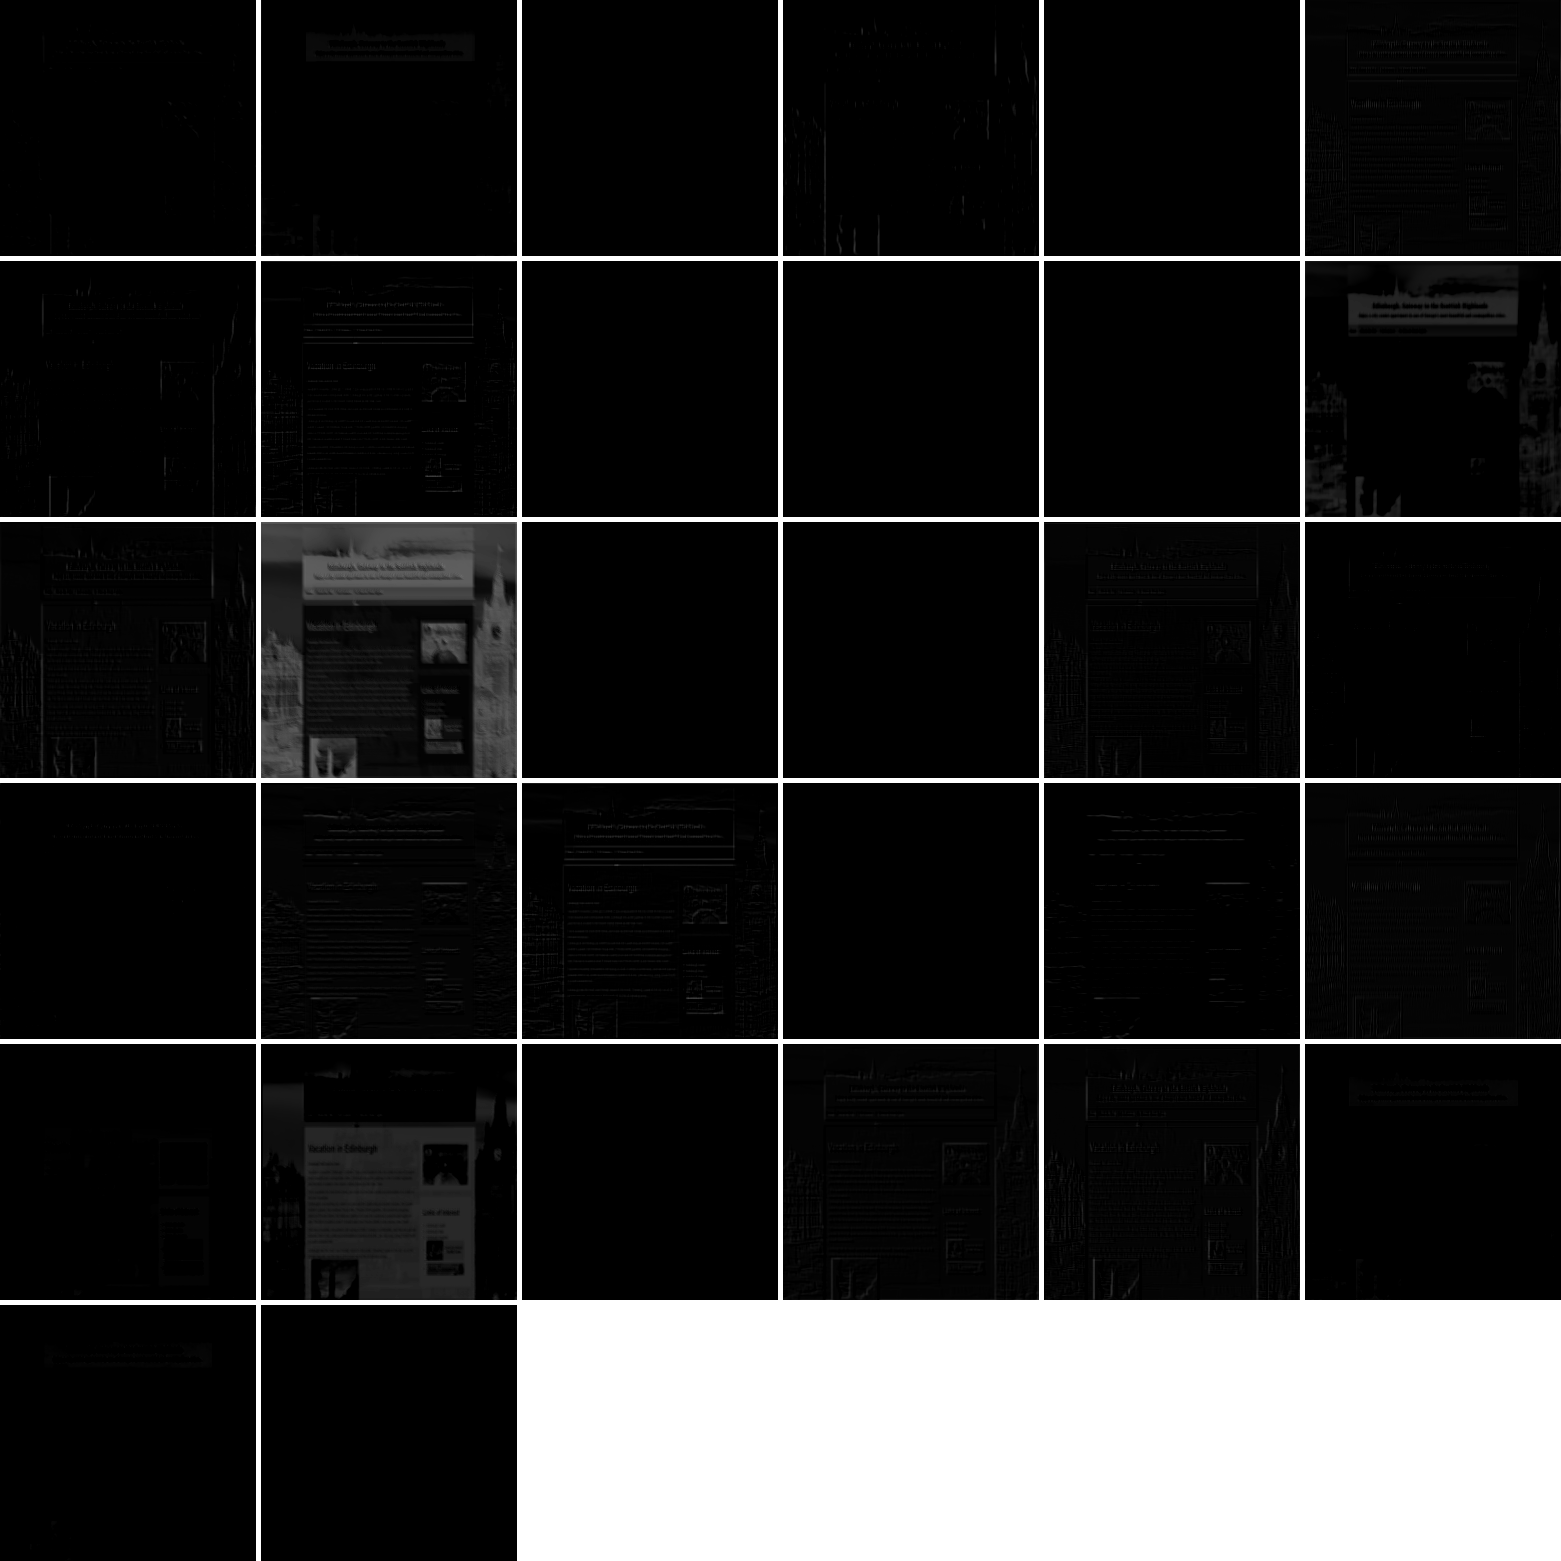
\includegraphics[width=0.6\columnwidth]{progettazione/feature_maps_layer_conv_1.png} 
  \caption{Feature map estratte dal primo strato convoluzionale}
  \label{fig:conv-1}
\end{figure}

\newpage

\begin{figure}[!htbp] 
  \centering 
  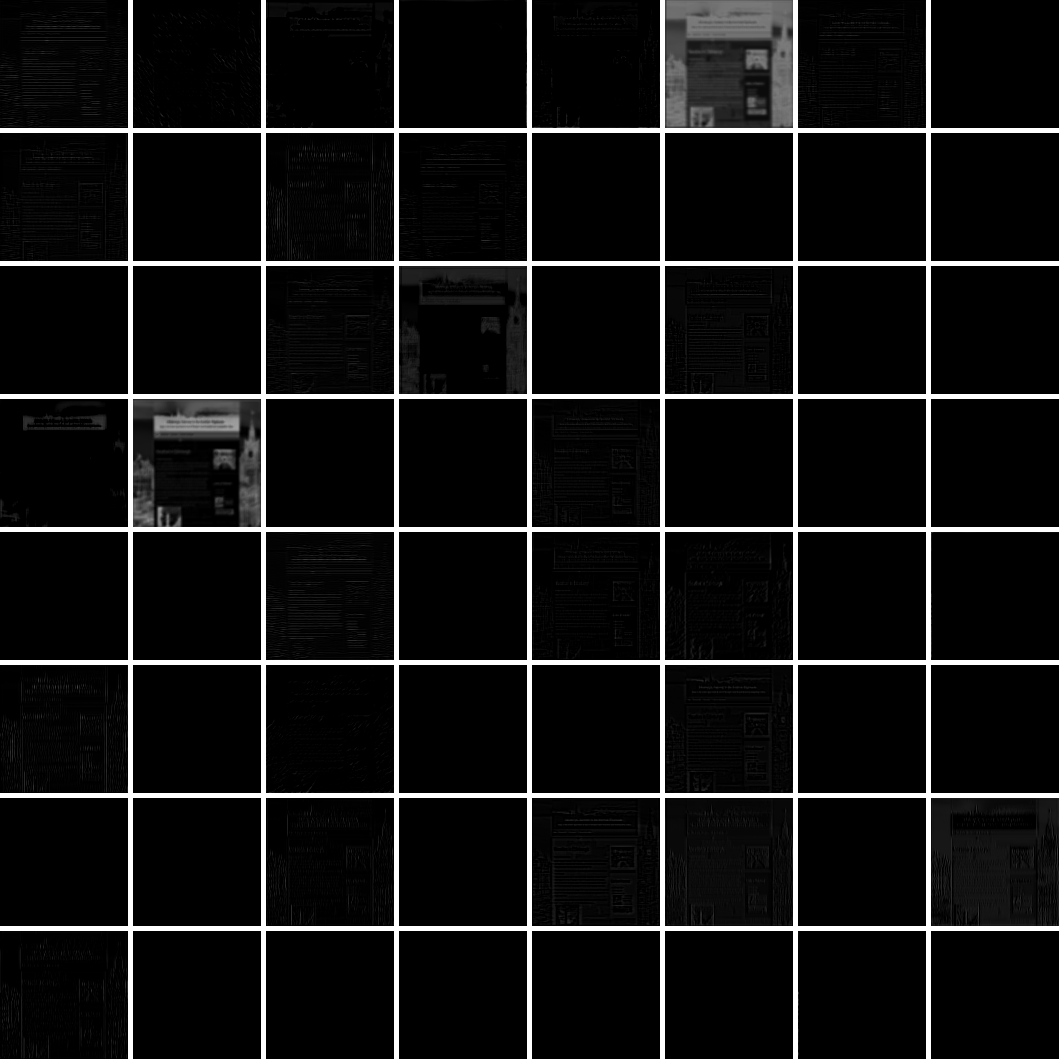
\includegraphics[width=0.6\columnwidth]{progettazione/feature_maps_layer_conv_2.png} 
  \caption{Feature map estratte dal secondo strato convoluzionale}
  \label{fig:conv-2}
\end{figure}

\begin{figure}[!htbp] 
  \centering 
  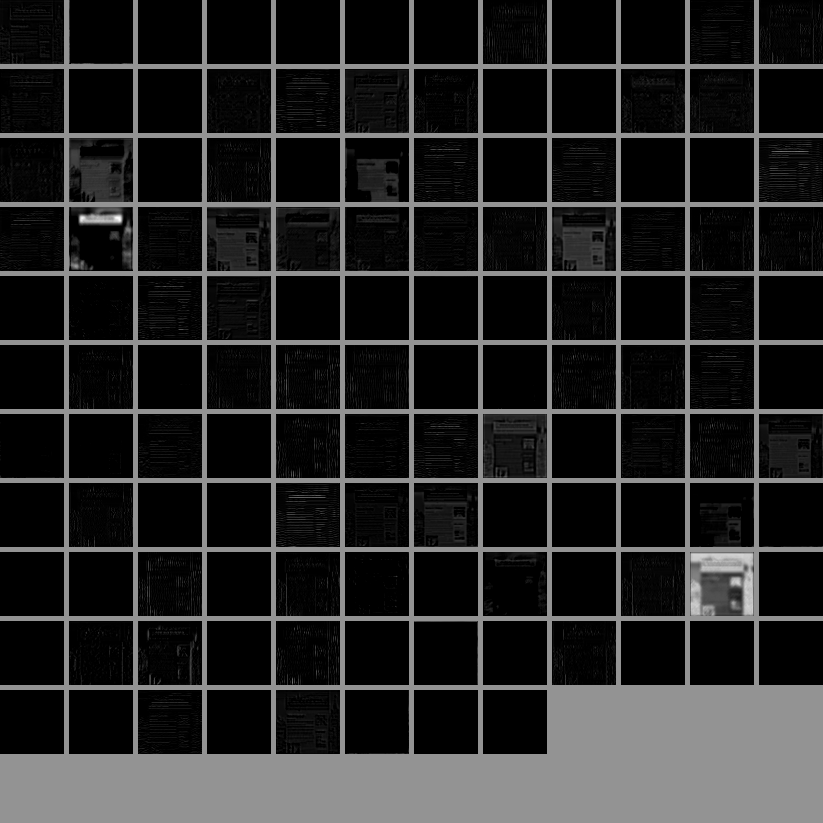
\includegraphics[width=0.6\columnwidth]{progettazione/feature_maps_layer_conv_3.png} 
  \caption{Feature map estratte dal terzo strato convoluzionale}
  \label{fig:conv-3}
\end{figure}

\newpage
Tramite l'utilizzo delle \emph{\gls{feature}} estratte dal \emph{bottleneck} è possibile effettuare un \emph{clustering} (Fig.~\ref{fig:cluster-conv})


\begin{figure}[!htbp] 
  \centering 
  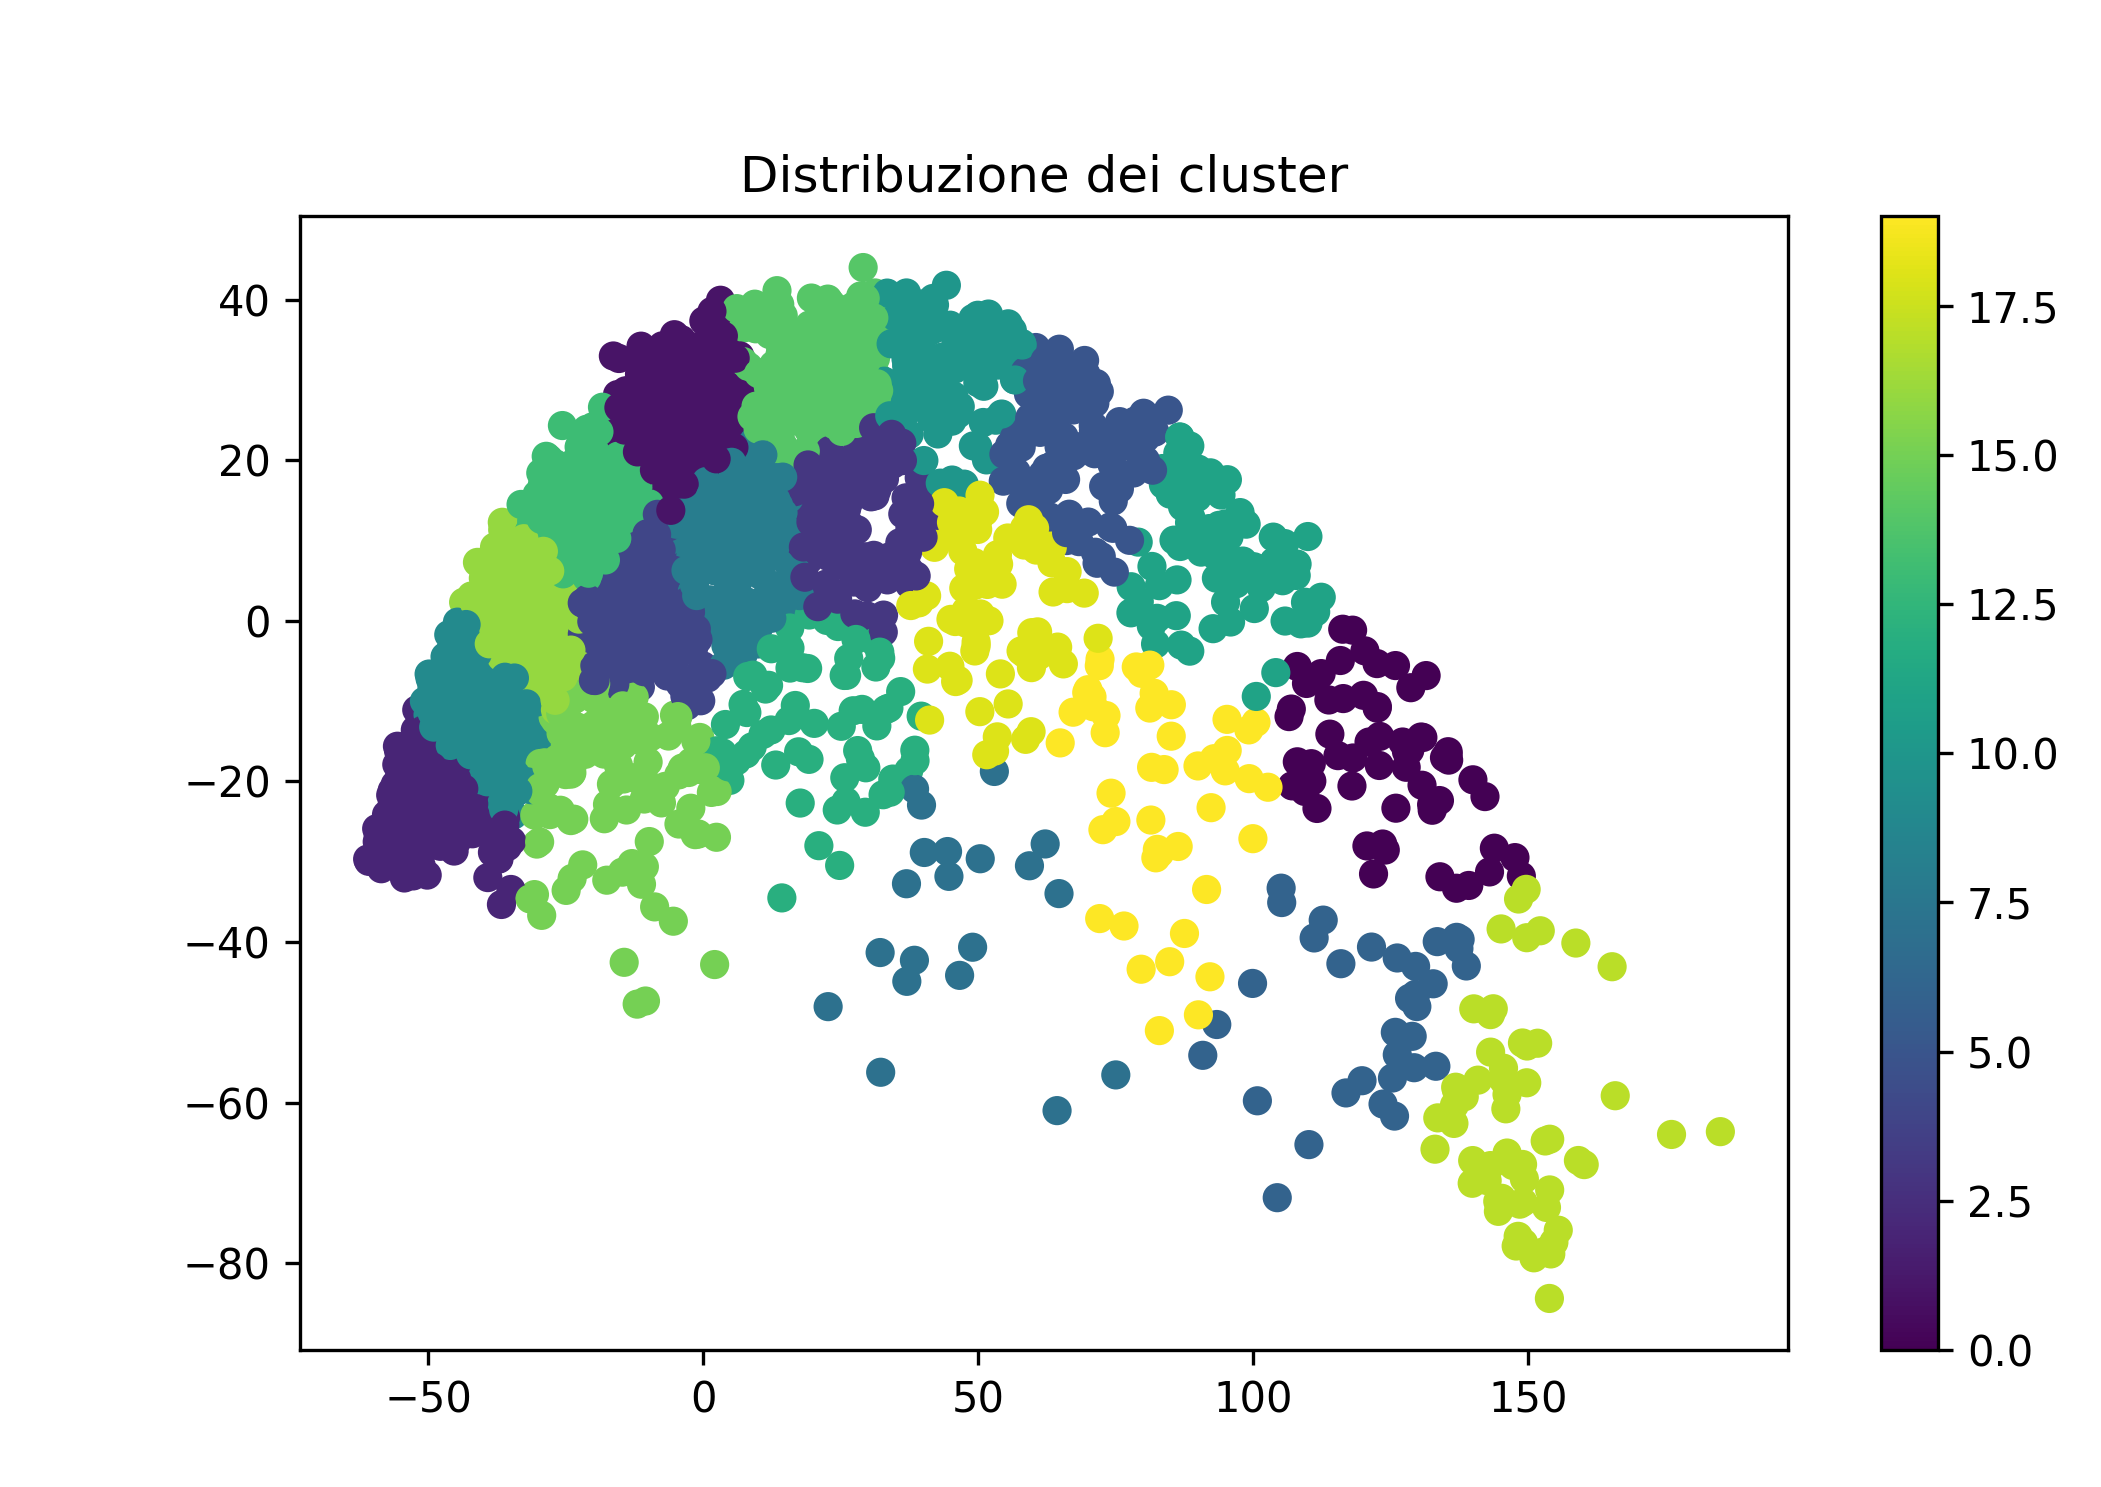
\includegraphics[width=0.7\columnwidth]{progettazione/Clusters_conv.png} 
  \caption{Clustering effettuato utilizzando le \gls{feature} estratte dall'autoencoder convoluzionale; 20 cluster e 3000 immagini}
  \label{fig:cluster-conv}
\end{figure}

\newpage

\subsection{Modelli pre-addestrati}
L'utilizzo di un modello preaddestrato consente di evitare la fase di addestramento e la complessa ingegnerizzazione di una rete neurale, per questo motivo l'utilizzo degli \emph{autoencoder} è stato scartato.
Il modello consigliato dal tutor è ResNet50, la scelta viene avvalorata dalle motivazioni riportate nell'articolo\footcite{site:why-resnet}:
\begin{itemize}
  \item Facillità di addestramento.
  \item Bilanciamento tra performance ed efficienza rispetto ad altri modelli della stessa famiglia.
  \item Risultati simili o migliori utilizzando meno risorse rispetto alla famiglia VGGNet. 
\end{itemize}

\section{Clustering}
\subsection{Preparazione delle immagini}
In seguito alla cattura le immagini vengono lette dal database e convertite in un formato utilizzabile dagli algoritmi di machine learning (Fig.~\ref{fig:schema-resize}).
Per velocizzare le operazioni in fase di addestramento tutte le immagini vengono scaricate dal database e convertite in formato PNG, poiché le librerie utilizzate necessitano di dati \emph{rester} per funzionare, successivamente le immagini salvate nella memoria del PC vengono processate in maniera tale da essere adatte all'utilizzo da parte di ResNet50.
In questo caso le dimensioni dei tensori richieste specificatamente dal modello (Fig.~\ref{fig:schema-tensore}) sono le seguenti (224*224*3):
\begin{itemize}
  \item Altezza dell'immagine
  \item Larghezza dell'immagine 
  \item Numero di canali (Red Green Blue)
\end{itemize}
Per rientrare nel formato richiesto le immagini subiscono un processo di \emph{scaling} che ne riduce la dimensionalità lasciando il contenuto invariato.
Tale operazione è stata preferita al \emph{cropping} perché utilizzandolo andrebbero a perdersi caratteristiche specifiche; ad esempio i margini bianchi ai lati del sito sono spesso segnale di un design un po'antiquato e migliorabile,  
la rimozione dei margini potrebbe compromettere il \emph{clustering} impedendo la creazione di un \emph{cluster} contenente pagine di quel tipo.
Inoltre ogni cella contiene valori compresi tra 0 e 255, per facilitare le operazioni tali valori vengono divisi per 255 e normalizzati in un intervallo compreso tra 0 e 1.

\begin{figure}[!h] 
  \centering 
  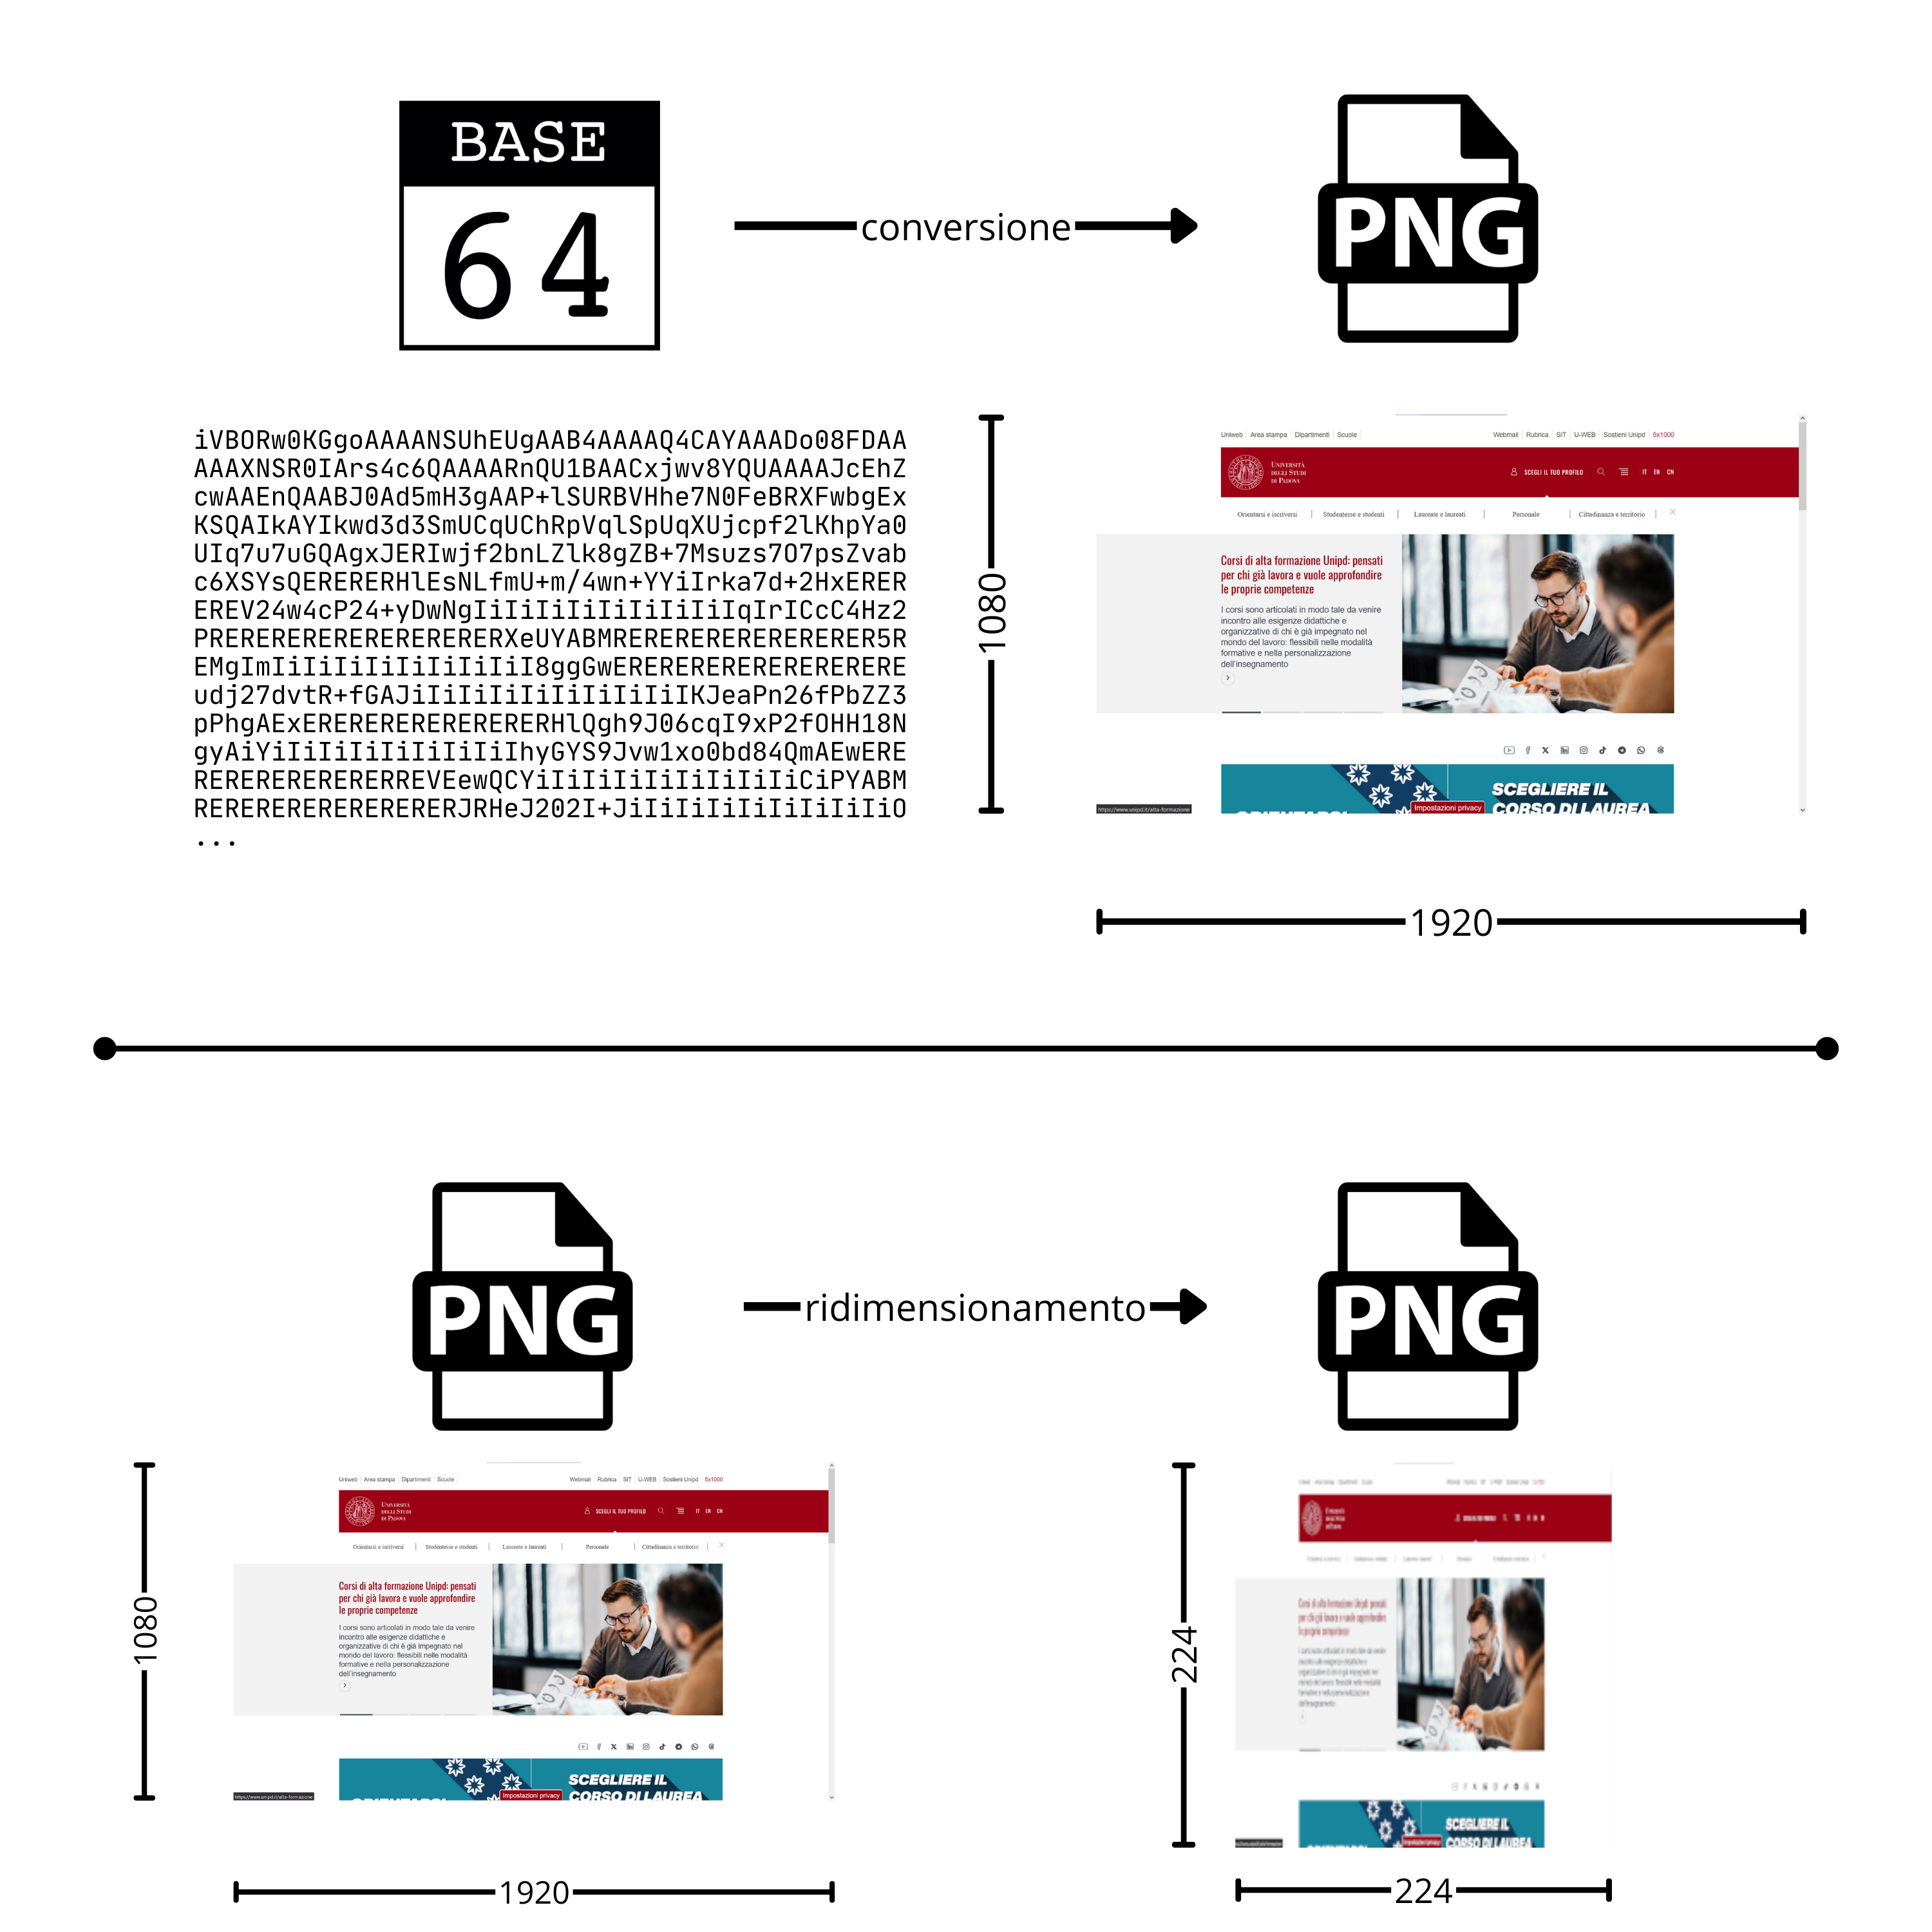
\includegraphics[width=0.7\columnwidth]{progettazione/schema-resize.png} 
  \caption{Conversione e ridimensionamento}
  \label{fig:schema-resize}
\end{figure}

\begin{figure}[!h] 
  \centering 
  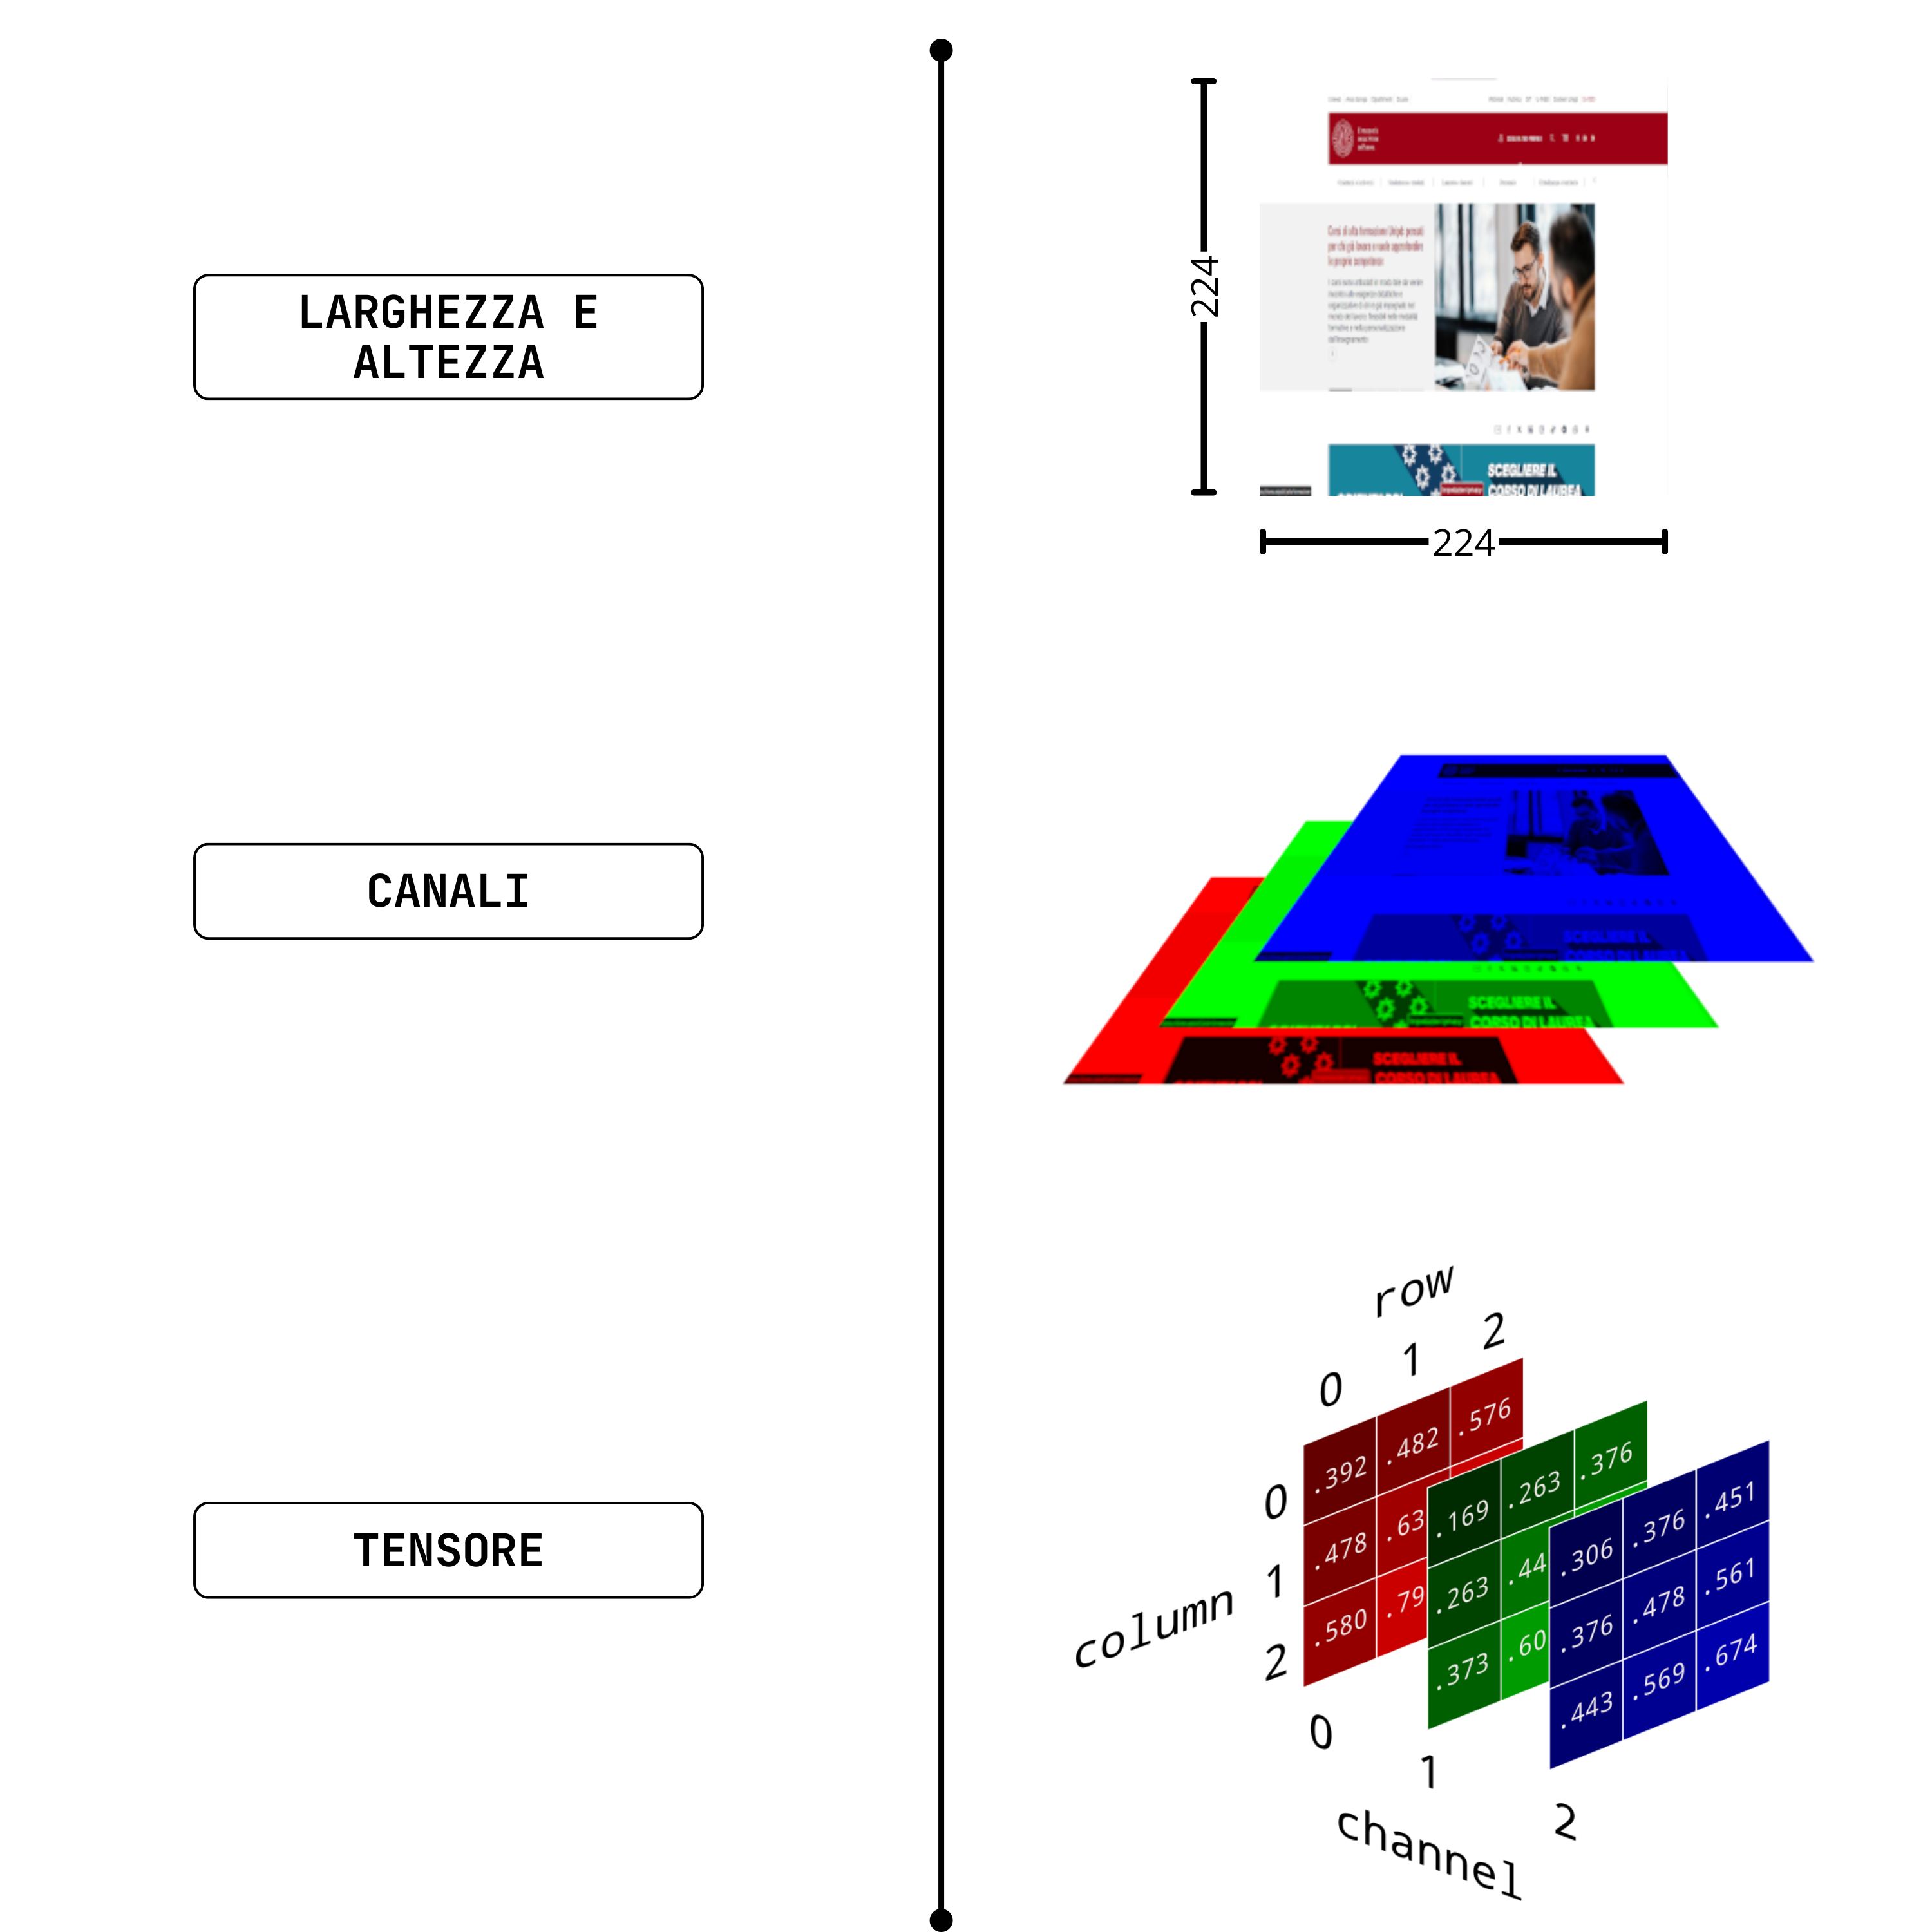
\includegraphics[width=0.5\columnwidth]{progettazione/schema-tensore.png} 
  \caption{Struttura del tensore}
  \label{fig:schema-tensore}
\end{figure}

\newpage


\subsection{Estrazione delle feature}
Per ottenere un dato utilizzabile in modo efficace dall'algoritmo di \emph{clustering} è necessario modificare ulteriormente le immagini riducendole a un set di \emph{\gls{feature}} (Fig.~\ref{fig:featuremaps}).
Per adempire a questo compito viene utilizzato un CNN Convolutional Neural Network pre-addestrato chiamato ResNet50 (Fig.~\ref{fig:schema-resnet}).
Il modello viene caricato senza i top \emph{layer}, ossia gli strati densi addetti alla classificazione, per sfruttare esclusivamente la sua abilità di riduzione in \emph{\gls{feature}}.

\begin{figure}[!h] 
  \centering 
  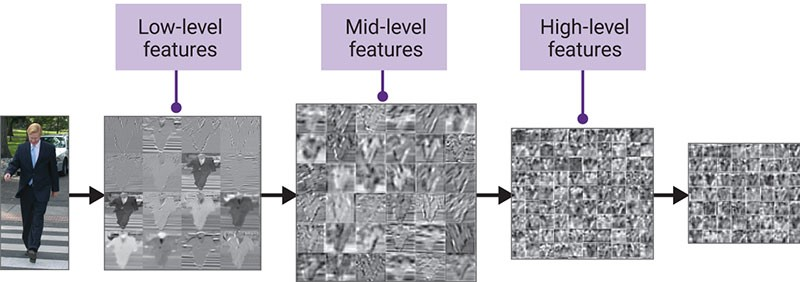
\includegraphics[width=0.7\columnwidth]{progettazione/esempio-featuremaps.png} 
  \caption{Esempio di feature maps}
  \label{fig:featuremaps}
\end{figure}

\begin{figure}[!h] 
  \centering 
  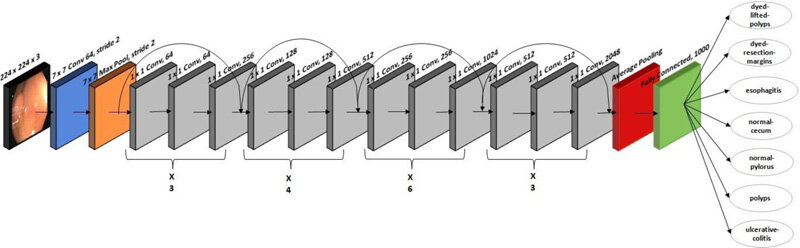
\includegraphics[width=0.9\columnwidth]{progettazione/schema-ResNet.png} 
  \caption{Struttura di ResNet50}
  \label{fig:schema-resnet}
\end{figure}



\subsection{Applicazione del clustering}
Le \emph{\gls{feature}} estratte dai \emph{layer} convoluzionali vengono ridotte a uno stato bidimensionale sfruttando l'analisi dei componenti principali, in questa maniera è possibile visualizzare i risultati del \emph{clustering} su un grafico cartesiano, ridurre i tempi di calcolo e aumentare l'accuratezza delle predizioni; ma al costo di una ovvia perdita di informazioni.
Successivamente viene applicato l'algoritmo dei K-means per l'effettiva suddivisione del \emph{\gls{dataset}} in \emph{cluster} (Fig.~\ref{fig:clusters-resnet}).
Le immagini vengono inserite, in base al \emph{cluster} a loro assegnato, nelle rispettive cartelle di appartenenza.
Questa operazione viene svolta per semplificare lo step successivo in cui lo sviluppatore deve preparare manualmente il \emph{\gls{dataset}} per l'addestramento supervisionato.

\begin{figure}[!h] 
  \centering 
  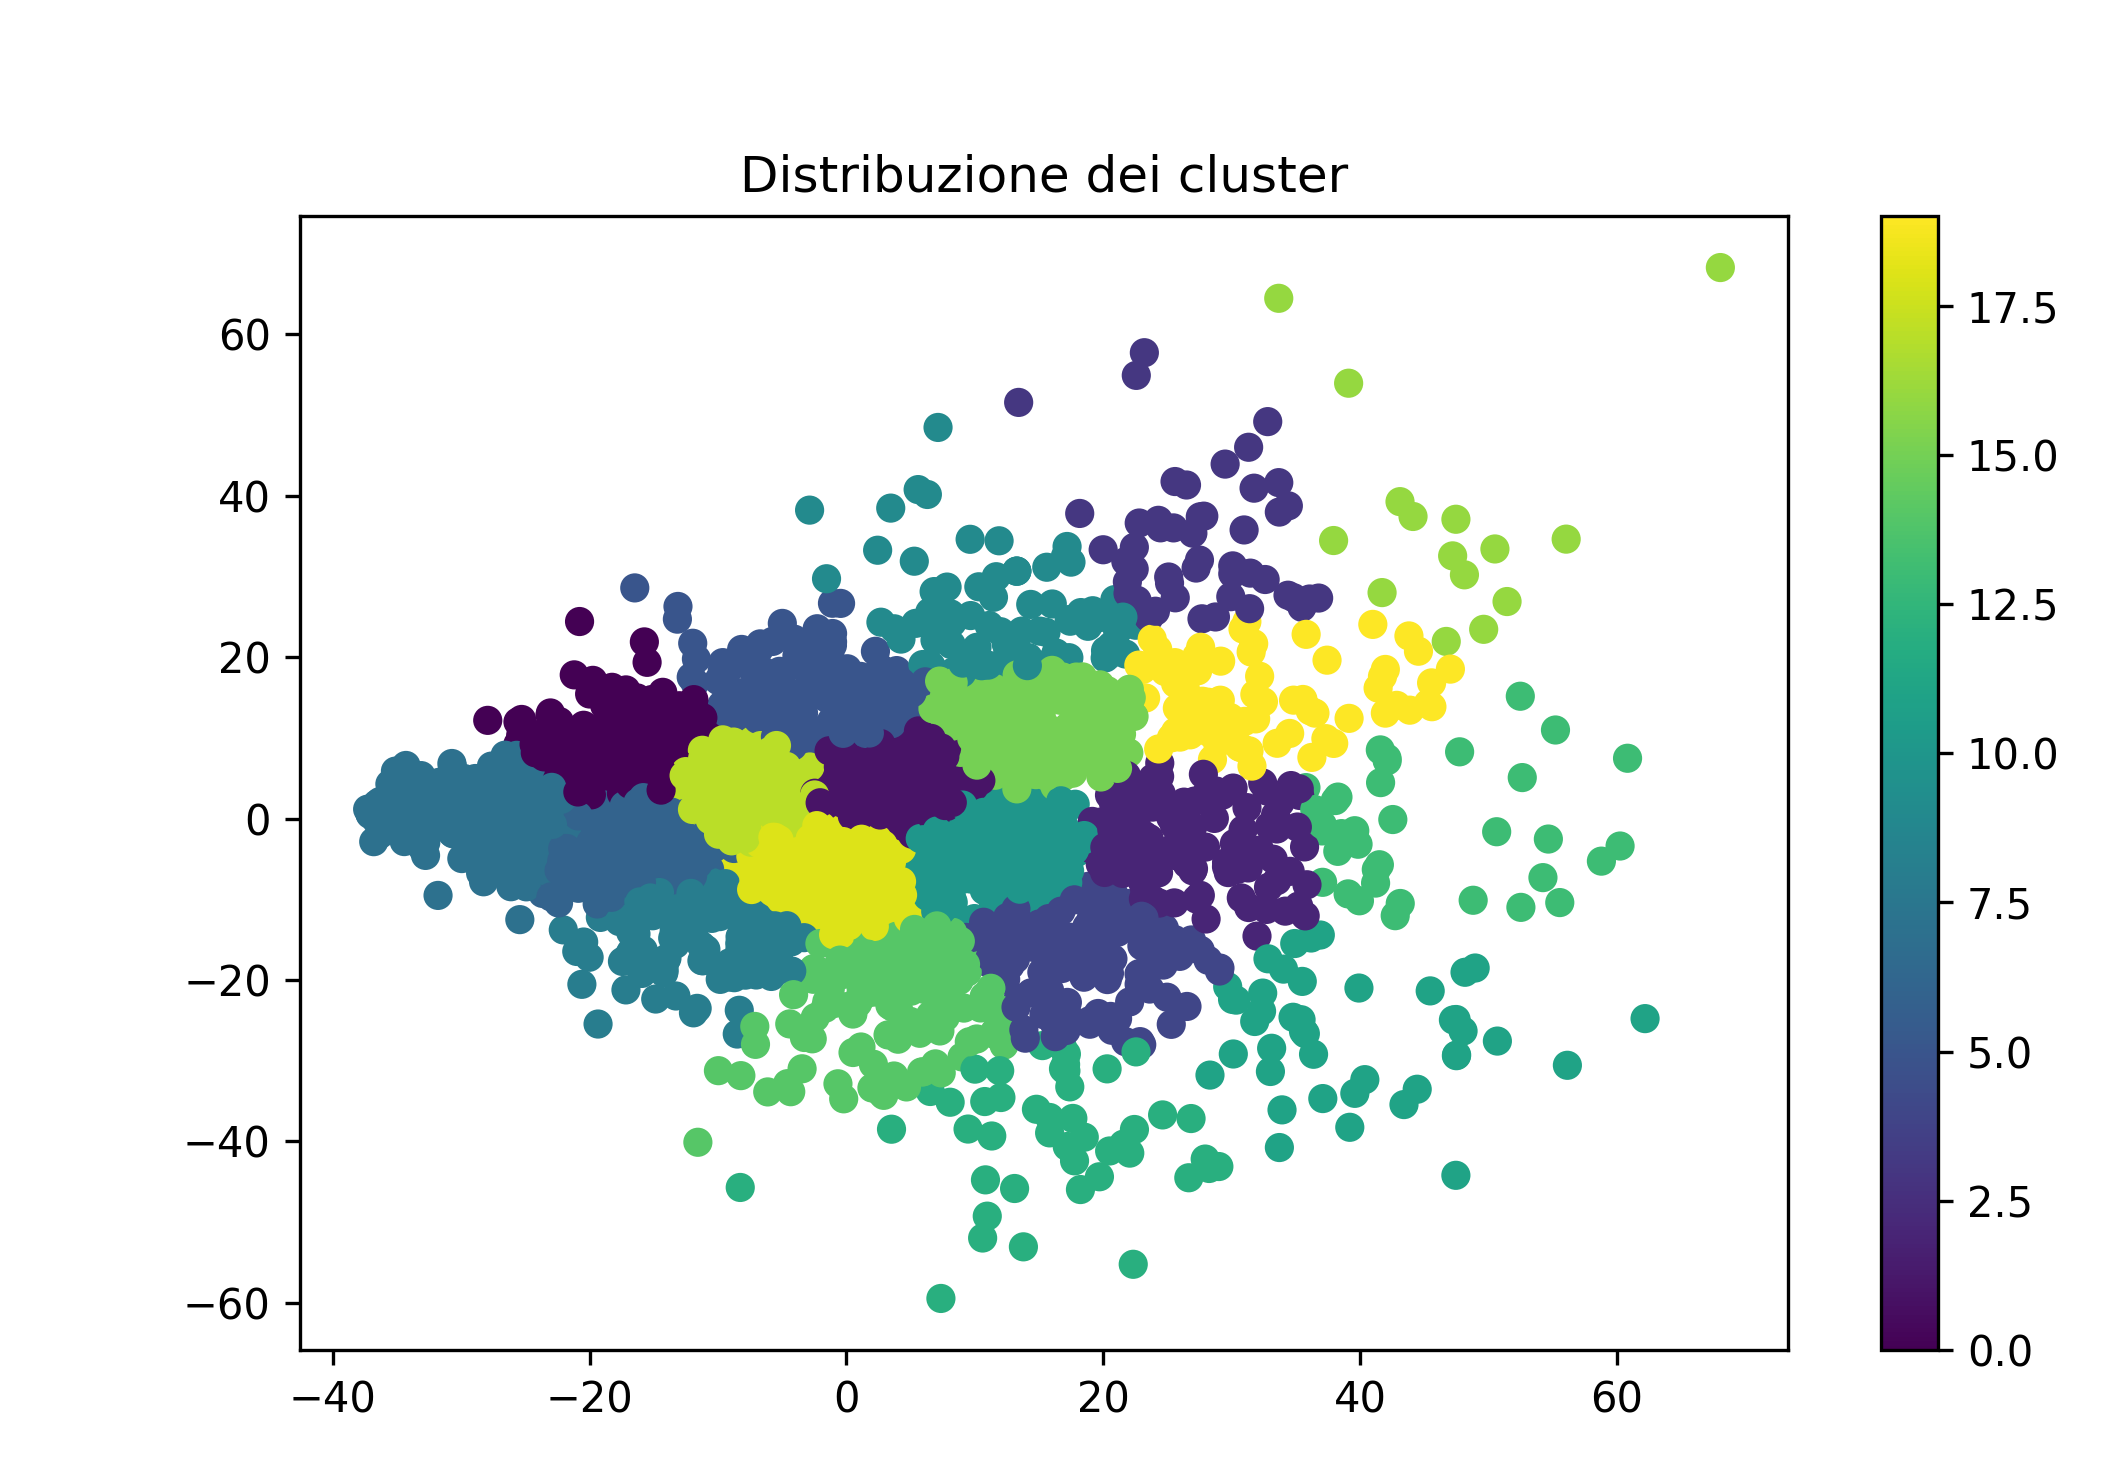
\includegraphics[width=0.7\columnwidth]{progettazione/Clusters-resnet.png} 
  \caption{Clustering effettuato utilizzando ResNet50; 20 cluster e 3000 immagini}
  \label{fig:clusters-resnet}
\end{figure}


%come modello finale è stato scelto resnet 50 poichè più rapido da utilizzare, infatti non necessita di addestramento 

\newpage

\section{Valutazione}

\subsection{Preparazione del dataset}
Il programmatore visiona i \emph{cluster} ottenuti precedentemente e verifica quali possono appartenere alle categorie "siti migliorabili" e "siti ottimi"; prepara due cartelle corrispondenti alle categorie e inserisce le immagini che reputa appartenere a ciascun dominio.
Lo script prepara il \emph{\gls{dataset}} (Fig.~\ref{fig:struttura-dataset}) secondo la logica seguente:
\begin{itemize}
  \item Training, il 70\% delle immagini viene utilizzato per l'addestramento effettivo.
  \item Validation, il 15\% delle immagini viene utilizzato per ottimizzare i parametri del modello.
  \item Test, il 15\% delle immagini serve per valutare l'\emph{output} del modello
\end{itemize}

\begin{figure}[!h] 
  \centering 
  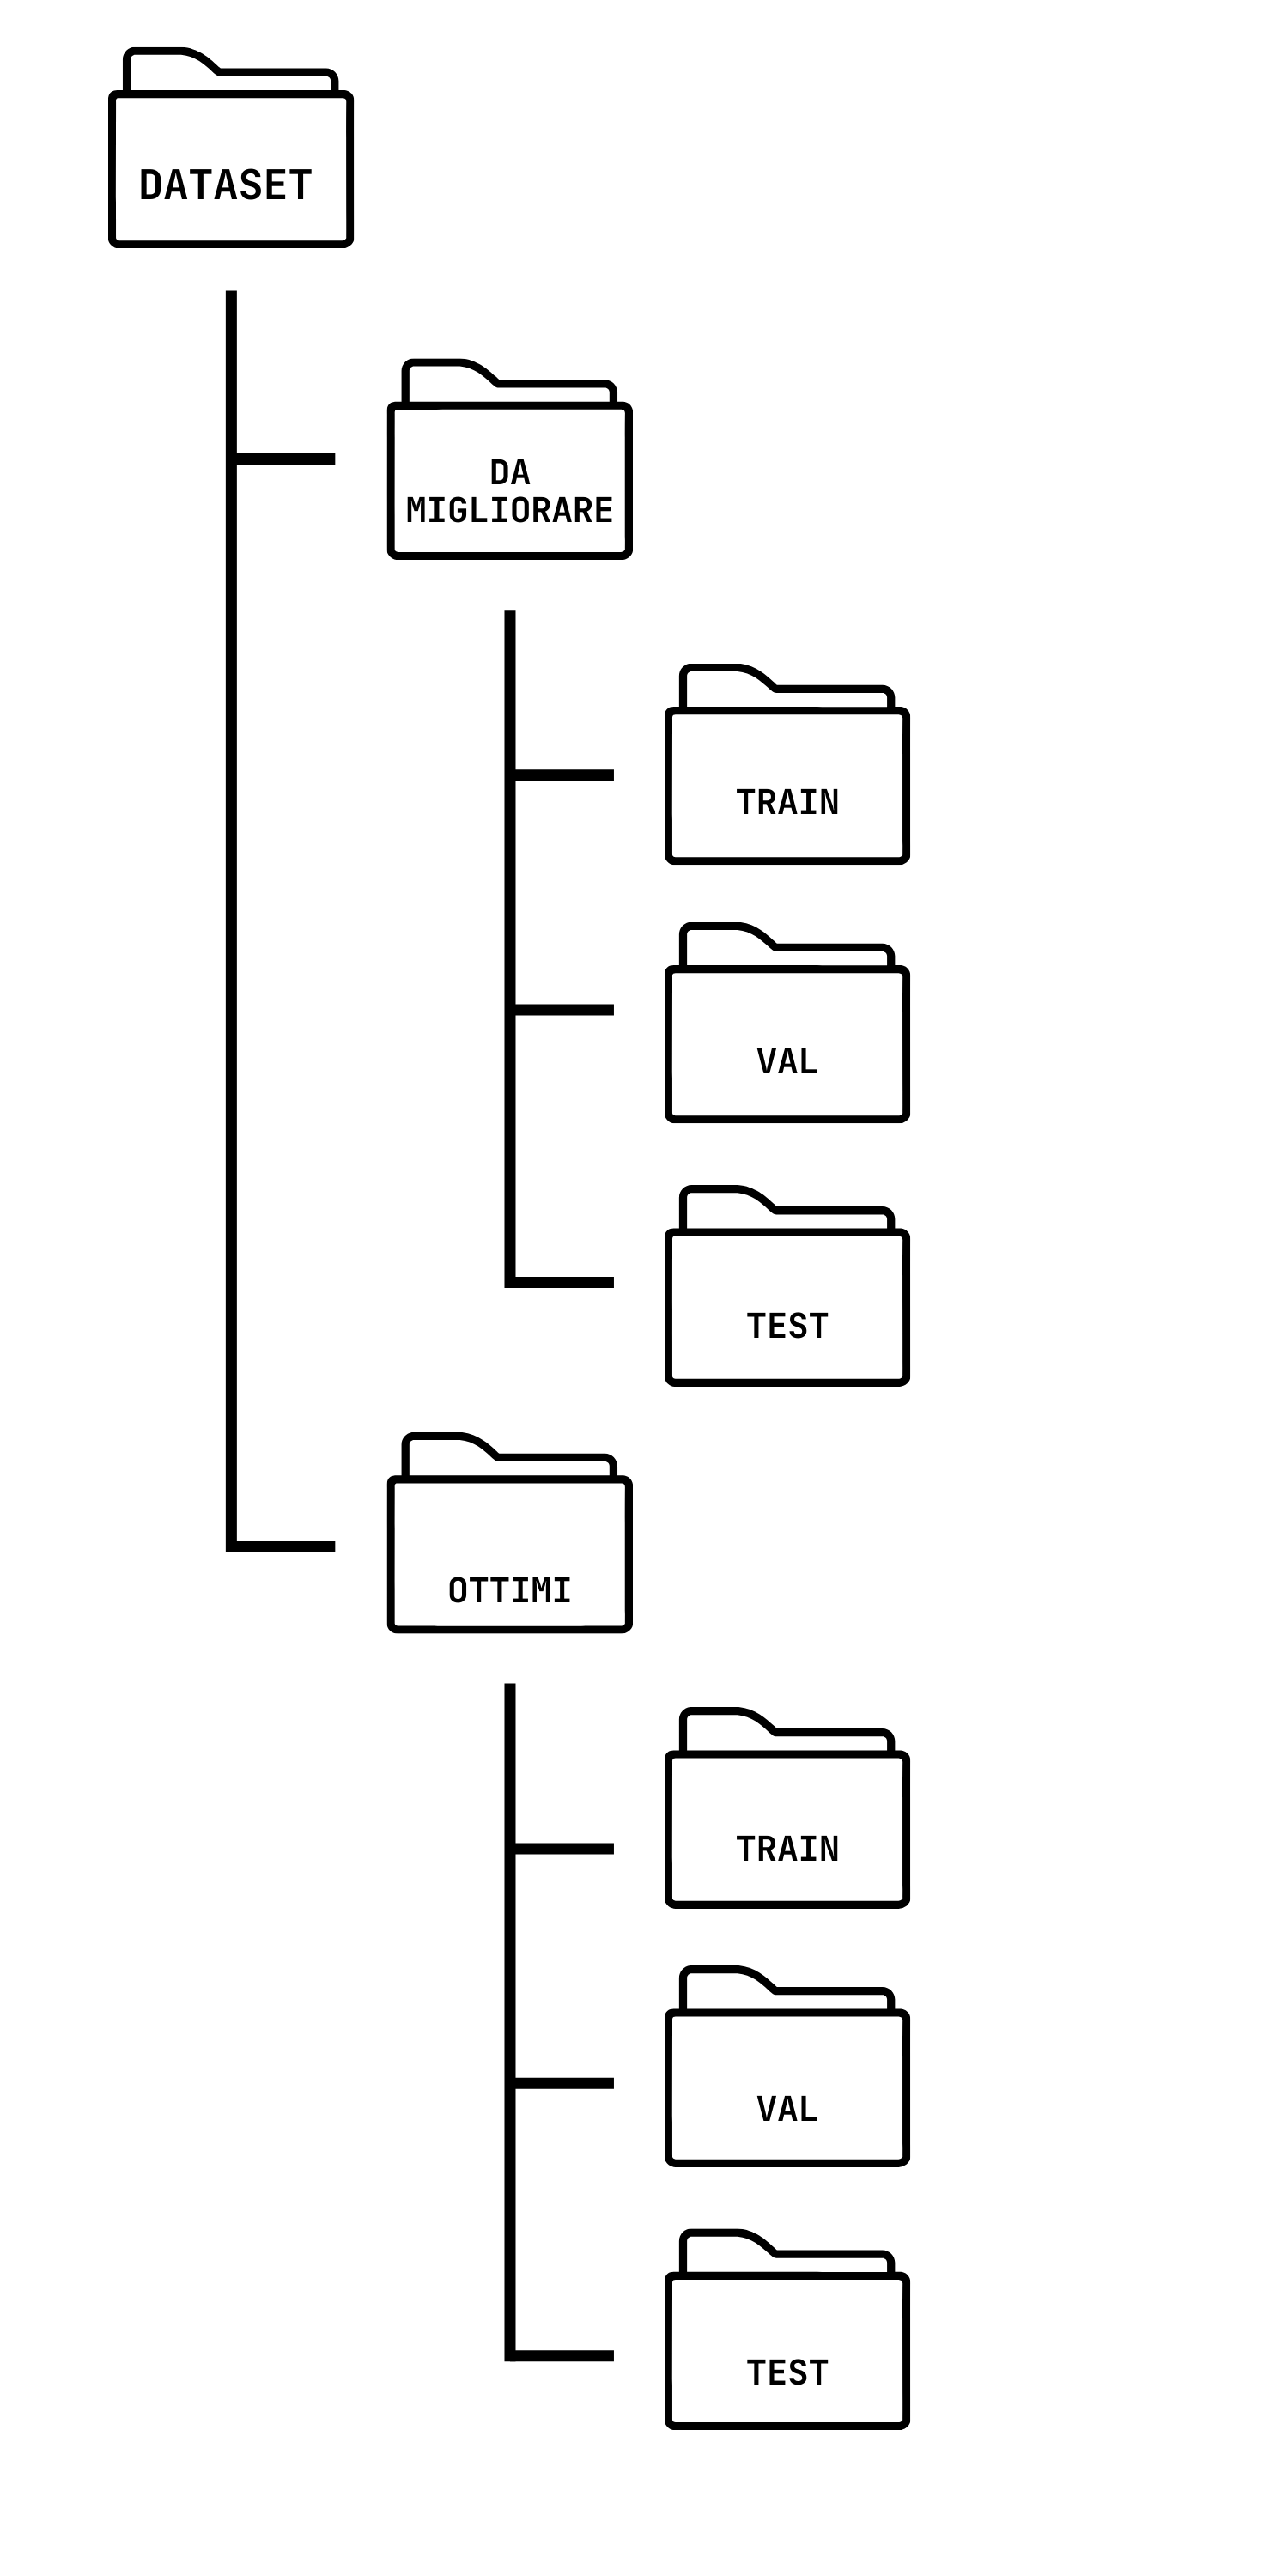
\includegraphics[width=0.35\columnwidth]{progettazione/struttura-dataset.png} 
  \caption{Struttura del dataset}
  \label{fig:struttura-dataset}
\end{figure}

\subsection{Addestramento del modello}
Viene caricato il modello pre-addestrato ResNet50 escludendo i \emph{top layer}, congelando i pesi e aggiungendo degli strati personalizzati per la classificazione.
Gli strati di classificazione sono successivamente addestrati utilizzando come \emph{input} le \emph{\gls{feature}} ricavate dai \emph{layer} convoluzionali congelati di ResNet50. 

\subsection{Fine-tuning del modello}
I \emph{layer} convoluzionali vengono sbloccati e il modello viene addestrato nuovamente nella sua interezza utilizzando un learning rate ridotto in maniera tale da non modificare completamente i pesi del modello preaddestrato.
Il modello viene salvato e riutilizzato ogniqualvolta sia necessario.

\subsection{Valutazione delle immagini}
Le immagini presenti nel database vengono classificate dal modello e le valutazioni in centesimi vengono restituite.

\section{Invio e-mail}
Le valutazioni vengono lette dal database e tramite Laravel si procede all'invio di mail personalizzate alle aziende che dispongono di siti web che potrebbero essere ancora migliorati.

\section{Database}
Il database di SalesCRM contiene molte tabelle ma in questa sezione vengono descritte solo quelle utilizzate dal \emph{\gls{workflow}}.

\subsection{Domains}
Questa tabella contiene tutte i siti web (Fig.~\ref{fig:schema-domains}) delle aziende collezionate dal \emph{web scraper} e le informazioni a essi correlati.


\begin{figure}[!h] 
  \centering 
  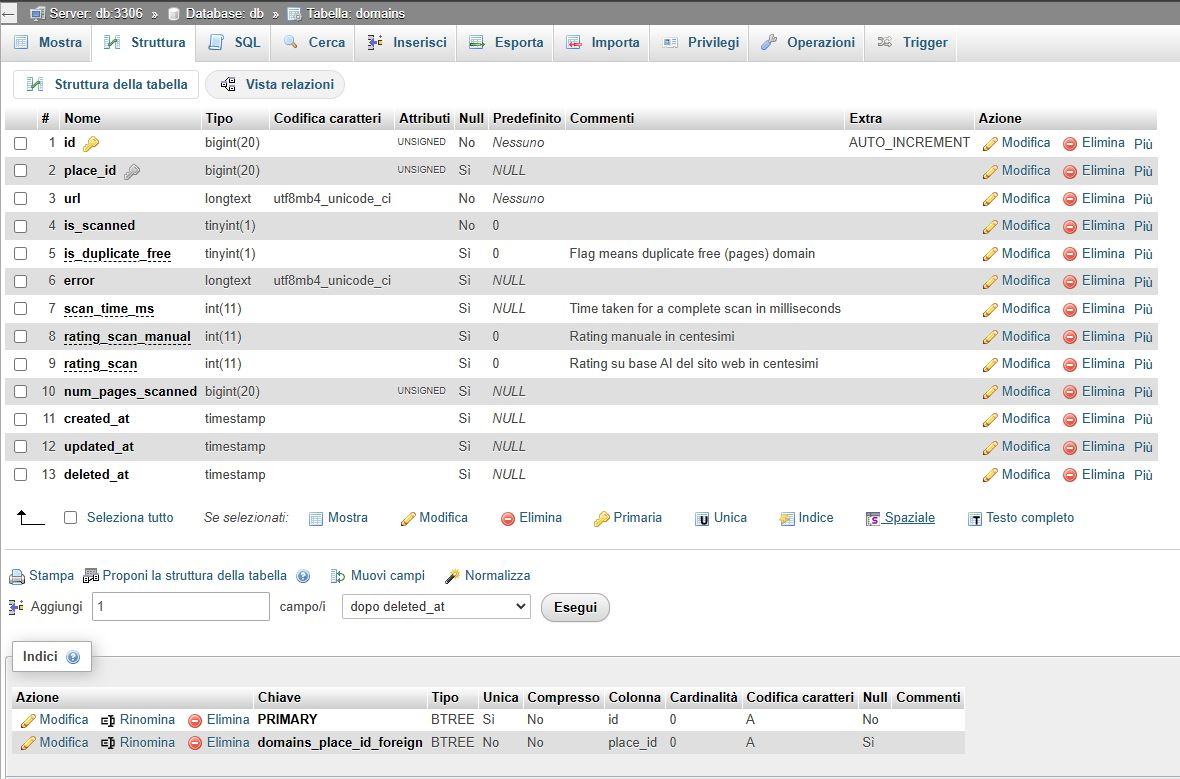
\includegraphics[width=0.9\columnwidth]{progettazione/schema-domains.png} 
  \caption{Schema della tabella Domains}
  \label{fig:schema-domains}
\end{figure}

\newpage 

\subsection{Pages}
Contiene i link a tutte le pagine (Fig.~\ref{fig:schema-pages}) di ciascun dominio.

\begin{figure}[!h] 
  \centering 
  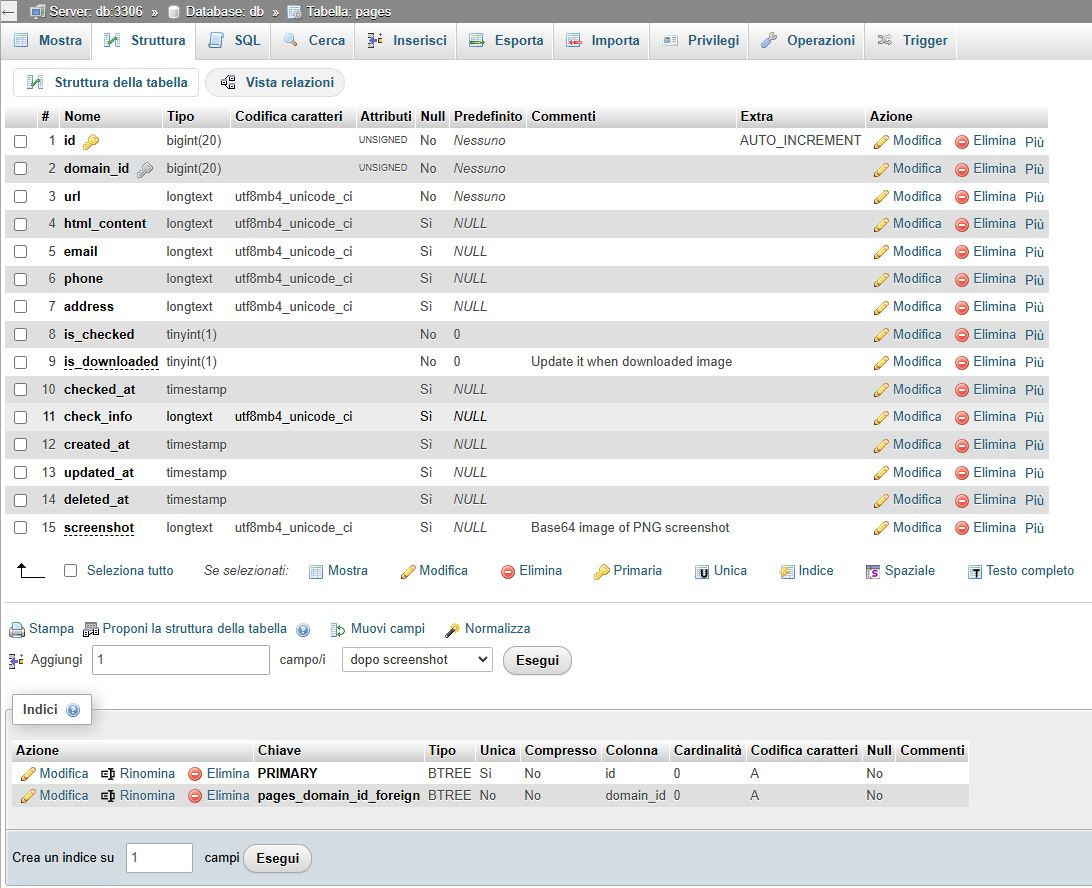
\includegraphics[width=0.9\columnwidth]{progettazione/schema-pages.png} 
  \caption{Schema della tabella Pages}
  \label{fig:schema-pages}
\end{figure}
